\documentclass[prd,twocolumn,nofootinbib,superscriptaddress,amsmath,amssymb]{revtex4-1}
\usepackage{mathtools}
\usepackage{graphics}
\usepackage{graphicx}
\graphicspath{{./images/}}
\usepackage{dcolumn}
\usepackage{bm}
\usepackage{dsfont} 
\usepackage{amsmath,amssymb}
\usepackage{hyperref}
\usepackage{tabularx}
%\usepackage{epstopdf}
\usepackage{epsf,epsfig}
\usepackage[normalem]{ulem}
\usepackage[usenames]{color}
\usepackage{multirow}
\usepackage{makecell}
\usepackage{diagbox}
\usepackage[abs]{overpic}
%\epstopdfsetup{outdir=./images/}
\allowdisplaybreaks
\hypersetup{
    colorlinks=true,
    linkcolor=blue,
    filecolor=magenta,      
    urlcolor=blue,
    citecolor=blue
}
\urlstyle{same}


\newcommand{\red}[1]{\protect\color{red} #1 \protect\color{black}}
\newcommand{\green}[1]{\protect\color{green} #1 \protect\color{black}}
\newcommand{\blue}[1]{\protect\color{blue} #1 \protect\color{black}}
\newcommand{\black}[1]{\protect\color{black} #1 \protect\color{black}}
\newcommand{\yellow}[1]{\protect\color{yellow} #1 \protect\color{black}}
\newcommand{\bra}[1]{\protect\langle #1 |}
\newcommand{\ket}[1]{| #1 \protect\rangle}
\newcommand{\braket}[2]{\protect\langle #1 | #2 \protect\rangle}
\newcommand{\expected}[1]{\protect\langle #1 \protect\rangle}
\newcommand{\R}{{\mbox{\tiny R}}}
\newcommand{\ky}[1]{\textcolor{blue}{\it{\textbf{ky: #1}}} }
\newcommand{\kent}[1]{\textcolor{magenta}{\textbf{ #1}} }
\newcommand{\zack}[1]{\textcolor{magenta}{\textbf{ #1}} }
\newcommand{\zc}[1]{\textcolor{red}{\it{\textbf{zc: #1}}} }
\definecolor{red(ncs)}{rgb}{0.77, 0.01, 0.2}
\newcommand{\ny}[1]{\textcolor{blue}{NY: #1} }
\newcommand{\kc}[1]{\textcolor{green}{KC: #1} }
\newcommand{\NS}{{\mbox{\tiny NS}}}
\newcommand{\sci}[2]{#1 \times 10^{#2}}

\usepackage{array}
\newcolumntype{C}[1]{>{\centering\let\newline\\\arraybackslash\hspace{0pt}}m{#1}}


\newcolumntype{C}[1]{>{\centering\arraybackslash}m{#1}}

\def\eq#1{Eq.~(\ref{eq:#1})}
\def\Eq#1{Equation~(\ref{eq:#1})}
\def\eqs#1#2{Eqs.~(\ref{eq:#1}) \& (\ref{eq:#2})}
\def\eqlist#1#2{Eqs.~(\ref{eq:#1}-\ref{eq:#2})}
\def\Eqs#1#2{Equations~(\ref{eq:#1}) \& (\ref{eq:#2})}
\def\Eqlist#1#2{Equations~(\ref{eq:#1}-\ref{eq:#2})}
\def\fig#1{Fig.\ref{fig:#1}}
\def\figs#1#2{Figs.\ref{fig:#1} \& \ref{fig:#2}}
\def\Fig#1{Figure~\ref{fig:#1}}
\def\Figs#1#2{Figures~\ref{fig:#1} \& \ref{fig:#2}}
\def\tab#1{Table~\ref{tab:#1}}
\def\sec#1{Section~\ref{sec:#1}}




\begin{document}

\title{EoS-insensitive relations after GW170817}

\author{Zachary Carson}
\affiliation{%
 Department of Physics, University of Virginia, Charlottesville, Virginia 22904, USA
}%

\author{Katerina Chatziioannou}
%\affiliation{%
% Canadian Institute for Theoretical Astrophysics, 60 St. George Street, Toronto, Ontario, M5S 3H8, Canada
%}%
\affiliation{%
 Center for Computational Astrophysics, Flatiron Institute, 162 5th Ave, New York, NY 10010
}%

\author{Carl-Johan Haster}
\affiliation{%
 Canadian Institute for Theoretical Astrophysics, 60 St. George Street, Toronto, Ontario, M5S 3H8, Canada
}%
\affiliation{%
 Center for Computational Astrophysics, Flatiron Institute, 162 5th Ave, New York, NY 10010
}%

\author{Nicol\`as Yunes}
\affiliation{%
 Department of Physics, Montana State University, Bozeman, MT 59717, USA.
}%
\affiliation{%
 Department of Physics and MIT Kavli Institute,
}%

\author{Kent Yagi}
\affiliation{%
 Department of Physics, University of Virginia, Charlottesville, Virginia 22904, USA
}%


\date{\today}

%%%%%%%%%%%%%%%%%%%%%%%%%%%%%%%% Begin Abstract %%%%%%%%%%%%%%%%%%%%%%%%%%%%%%%%%%%%%%%%%%%%%%%%%%%%%%%%%%%%%%%%%%%%%%%%%%%%%%%%%%%%%%%%%%%%%%%%%%%%%%%%%%%%%%%%%%%%%%%%%%%%%%%%%%%%%%%%%%%%%%%%%%%%%%%%%%%%%
\begin{abstract}
% Intro
The thermodynamic relationship between pressure and density (the equation of state, or EoS) of cold supranuclear matter, accessible in neutron stars, is critical to the study of such stars, and is one of the largest uncertainties in nuclear physics to date. 
% How to probe
The extraction of tidal deformabilities from the gravitational waveforms of binary neutron star merger events, such as GW170817, is a promising method of probing the nuclear structure.
% What was done before - Binary Love
Previous studies have shown that approximately EoS-insensitive ``binary Love relations" exist between symmetric and antisymmetric combinations of individual tidal deformabilities, which are difficult to be independently measured with second-generation gravitational wave interferometers.
% What was done before - I-Love-Q
Similarly, another set of EoS-insensitive relations exist between individual neutron star parameters: moment of inertia (I), tidal deformability (Love number), quadrupole moment (Q), and compactness (C) - known as the ``I-Love-Q" and ``C-Love" relations.
% What universal relations do
Such EoS-insensitive relations allow the elimination of some tidal parameters from the list of model parameters, thus breaking degeneracies and ultimately reducing parameter extraction uncertainties.
% What we will do
However, even the most precise of EoS insensitive relations carry EoS variation which inject systematic errors into the parameter extraction process.
In this document, we explain how one can reduce equation of state variation for I-Love-Q, C-Love, and binary Love relations, which helps to reduce systematic errors on the tidal measurement of binary neutron star mergers.
However, we show that the systematic effects of these relations is very small until next-generation detectors. 
We achieve this  by restricting to only equations of state drawn from the 90\% posterior constraint on pressure as a function of density, as derived by the LIGO Collaboration.
% What we found
We find an improvement in binary Love universality by a factor of $\sim 59$\% for stars with a mass ratio of 0.75, in C-Love universality by a factor of $\sim 67\%$, and in I-Love-Q universality by factors of $\sim 50$\%.
% Conclude
We end by comparing systematic errors on tidal measurement due to the equation of state variation with statistical errors and comment on whether one can safely use these EoS-insensitive relations with future gravitational wave observations.
We conclude that the systematic errors injected from the use of improved EoS-insensitive relations become comparable to the statistical errors for future design upgrade Voyager.
\end{abstract}

\maketitle

%%%%%%%%%%%%%%%%%%%%%%%%%%%%%%% Begin Introduction %%%%%%%%%%%%%%%%%%%%%%%%%%%%%%%%%%%%%%%%%%%%%%%%%%%%%%%%%%%%%%%%%%%%%%%%%%%%%%%%%%%%%%%%%%%%%%%%%%%%%%%%%%%%%%%%%%%%%%%%%%%%%%%%%%%%%%%%%%%%%%%%%%%%%%%%%%%%%%

\section{Introduction}\label{sec:intro}
%Intro

{\ny{Just some general comments so that we don't forget:
\begin{itemize}
\item The EoS-insensitive relations are called ``binary Love'', ``I-Love-Q'', ``C-Love'' and ``R-Love.'' There is no need to call them ``binary Love EoS-insensitive relations.'' That's too verbose and not what they are called in the literature. I am ok with describing these relations as EoS-insensitive instead of approximately universal, but let's not change the names. 
\item There is some serious tidying up that needs to be done to all of the text. Specifically, there are missing prepositions, like ``the'', in lots of places that makes the reading a bit choppy and we can improve. Zack, when you have a chance, please do a detail read through and fix the flow as much as you can. 
\item Eventually, we need to discuss the abstract and the intro in more detail. 
\item Let's not forget to check the acknowledgements for funding sources. 
\item Let's do a spell check. 
\item Let's remove all commented out text.  
\end{itemize}
}}
The dependence of pressure on density for cold supranuclear matter found inside neutron stars (NSs) remains to be one of the largest mysteries in both nuclear physics and astrophysics.
This internal structure of such stars, known as the equation of state (EoS), is exceedingly important, as it is the determining factor for many NS observables - such as the mass, the radius, and many more.
Unfortunately, terrestrial experiments can only study the EoS to around the nuclear saturation density ($\rho_{\text{sat}} \approx 2.5 \times 10^{14} \text{ g/cm}^3$)~\cite{Li:HeavyIon,Tsang:SymmetryEnergy,Centelles:NeutronSkin,Li:CrossSections,Chen:SymEnergy} (although some temperature-dependent heavy-ion collision experiments may probe higher densities \zc{Katerina do you know of any papers on this?} {\ny{Look up the PREX and CREX experiments at JLab (a good author is Horowitz, e.g. Abrahamyan:2012gp, Horowitz:2012tj, Horowitz:2013wha)}}), making NSs ideal laboratories for constraining ultra dense nuclear matter.

%Constraining the EoS
Independent measurements of NS observables can be used to constrain the nuclear EoS.
For example, electromagnetic observations of the mass-radius relationship of NSs have been used to place limits on the NS EoS~\cite{guver,ozel-baym-guver,steiner-lattimer-brown,Lattimer2014,Ozel:2016oaf}.
However, these implications potentially suffer from large systematic errors due to various x-ray burst astrophysical mismodeling uncertainties.
Alternatively, the emission of gravitational waves (GWs) from binary NS merger events have proven to be a unique method of probing nuclear physics.
During the early inspiral portion of the merger, the orbital separation is large enough that the effect of companion tidal fields is negligible. 
As the separation decreases through GW emission, tidal forces are magnified and the NSs deform from sphericity, altering the orbital trajectories; a relic which is directly imprinted on the GW signal.
This deformation is characterized by the \textit{tidal deformability} $\Lambda$ as the linear response of the NSs quadrupole moment $Q_{ij}$ to the neighboring tidal field $\varepsilon_{ij}$~\cite{hinderer-love,Flanagan2008}.

%reparameterization of the template
In the case of binary NSs, each star becomes deformed via the process highlighted above, resulting in two highly correlated tidal parameters $\Lambda_1$ and $\Lambda_2$ entering in the gravitational waveform\cite{Flanagan2008,Vines:2011ud}.
Due to high correlations between between the two parameters, independent extraction becomes very difficult at current interferometer sensitivities~\cite{Wade:tidalCorrections}.
Typically, these high correlations can be reduced by strategically reparameterizing the waveform template with new tidal parameters constructed from linear combinations of $\Lambda_1$ and $\Lambda_2$.
For example, utilizing the parameters $\tilde{\Lambda}$ and $\delta \tilde{\Lambda}$~\cite{Favata:2013rwa,Wade:tidalCorrections} which enter the GW waveform at different post-Newtonian (PN) orders (powers of the ratio between the orbital speed and the speed of light $v/c^{2n}$) partially mitigates these correlations.
Similarly, the waveform may be parameterized by mass-independent tidal parameters $\lambda_0$ and $\lambda_1$, derived through a Taylor expansion about $m_0=1.4 \text{ M}_{\odot}$ of individual, unitful tidal deformability $\lambda \approx \lambda_0+\lambda+1(m_1-1.4 \text{ M}_{\odot})/\text{M}_{\odot}$~\cite{delPozzo:TaylorTidal}. 
Use of this set of tidal parameters allows one to effectively combine multiple events with varying mass and $\tilde\Lambda$ components, not possible in the former parameterization of $\tilde{\Lambda}$ and $\delta \tilde{\Lambda}$

%Universal relations
Unfortunately, current detectors are only sensitive enough to accurately measure the dominant tidal parameter, $\lambda_0$.
Previous work by Yagi and Yunes~\cite{Yagi:binLove} resolved this issue by finding approximately EoS-insensitive ``binary Love universal relations" between symmetric and anti-symmetric combinations of tidal deformabilities $\Lambda_{s,a}=\frac{1}{2}(\Lambda_1 \pm \Lambda_2)$.
This allows one to further break degeneracies between tidal parameters, resulting in both (i) a decrease in uncertainty upon parameter extraction of $\Lambda_s$ on the removal of parameter $\Lambda_a$ from the model, and (ii) the ability to measure the secondary tidal parameter upon measurement of the first~\cite{Katerina:residuals}.  
Use of these relations leads to up to an order of magnitude improvement in parameter estimation of $\Lambda_s$ through a simple Fisher analysis~\cite{Yagi:binLove}, also confirmed with the detailed analysis of~\cite{Katerina:residuals}.
Similar ``I-Love-Q" and ``C-Love" relations~\cite{Yagi:ILQ} have been found between individual NS observables: quadrupole moment , moment of inertia, tidal deformability, and compactness; similarly allowing the removal of tidal parameters from the model list, and allowing an automatic determination of one observable through the measurement of another.
However, these EoS-insensitive relations have been tuned to a collection of EoS models, and each have intrinsic uncertainties associated with their use.

%How we improved this
In this analysis, we aim to improve this important work by imposing the restrictions found on the EoS~\cite{LIGO:posterior} derived from the recent binary NS merger observation, GW170817~\cite{TheLIGOScientific:2017qsa}.
By restricting to only EoSs which lie within the the 90\% credible region on pressure as a function of density found in~\cite{LIGO:posterior}, we repeat the analyses done in~\cite{Yagi:binLove,Yagi:ILQ} and show an increase in universality for I-Love-Q, C-Love, and binary Love relations.
We also investigate the relationship between the NS radius and its tidal deformability, or the R-Love relations, determining if the uncertainties can be reduced.
In addition, we consider hybrid star EoSs seen in~\cite{Paschalidis2018}, which experience strong first-order transitions from hadronic matter to quark matter.
These provide a departure from the nuclear matter relations considered here - providing valuable insight into them.
Further, we estimate the viability of using improved EoS-insensitive relations on future GW detections by performing simple Fisher analyses to approximate when the statistical errors from parameter extraction become comparable to the systematic errors due to EoS variation in EoS-insensitive relations.
To estimate the effect of waveform mismodeling, we additionally consider two different tidal corrections to the injected PhenomD~\cite{PhenomDI,PhenomDII} waveform: 6PN~\cite{Wade:tidalCorrections} and NRTidal~\cite{Samajdar:NRTidal}

\subsection{Executive Summary}
\zc{Me and Kent discussed whether or not we should include this section or not, and we decided like having the quick summary for busy readers - especially with the increasing number of figs and tables (8 tables, 14 figures so far). We can discuss this further if anyone doesn't want it included :)}
{\ny{I'm ok with keeping this, but let's get the science finished first.}}
%What we did
In this paper we attempt to improve I-Love-Q, C-Love, and binary Love relations by imposing constraints on the EoS found by GW170817~\cite{LIGO:posterior,TheLIGOScientific:2017qsa}.
First, we generate two large samples of spectral EoSs~\cite{Lindblom:2018rfr}, where we (i) impose the restriction that they must be drawn from GW170817s 90\% credible posterior in pressure as a function of density, and (ii) don't impose any restrictions for comparison purposes.
Next, we follow the important works of~\cite{Yagi:binLove} and~\cite{Yagi:ILQ} to show how the ``constrained" set of EoSs show improved universality (binary Love, I-Love-Q, and C-Love) from both the previous works, and the ``unconstrained" sample, shown by Fig.~\ref{fig:ILQ}.
In addition, we determine the degree to which hybrid star EoSs obey binary Love relations.
Finally, through a simple Fisher analysis, we consider the value in improving EoS-insensitive relations by approximating when the statistical errors from parameter extraction become comparable to the systematic errors due to EoS variation in EoS-insensitive relations.

%Final Results
Upon use of the constrained set of EoSs, we find an improvement in binary Love universality by a factor of $\sim 59$\% for stars with mass ratios of $0.75$, in C-Love universality by a factor of $\sim 67\%$, and in I-Love-Q universality by factors of $\sim50$\%, tabulated in Tab.~\ref{tab:maxVar}.
We also present new R-Love relations displaying the relationship between NS radius and tidal deformability, showing maximum EoS variability of $18.88\%$ from the fit discussed in Sec.~\ref{sec:clove}.
Additionally, we find that hybrid quark-hadron stars do obey the I-Love-Q and C-Love relations, with sightly increased EoS variability.
We also find that binaries consisting of one massive hybrid star, and one small-mass hadronic star do not agree with derived binary Love relations, due to the large separation in $\tilde{\Lambda}$ between the constituent stars.
Due to the current limitations in detector sensitivity, the systematic errors arising from EoS variation in the EoS-insensitive relations are far outweighed by the statistical errors accrued by extraction of high-order PN tidal parameters from GW waveforms.
Fig.~\ref{fig:stackedFisher} compiles the results from Fisher analyses approximating the uncertainties accrued from parameter extraction for GW170817 as if it had been observed by future detectors $A \equiv ($ O2~\cite{aLIGO}, aLIGO~\cite{aLIGO}, A\texttt{+}~\cite{Ap_Voyager_CE}, Voyager~\cite{Ap_Voyager_CE}, ET~\cite{ET}, CE~\cite{Ap_Voyager_CE}$)$.
Here, $\sigma^A_{\text{GW170817}}$ and $\rho^A_{\text{GW170817}}$ correspond to the statistical error and signal-to-noise-ratio found from observing GW170817 on detector $A$, and $\sigma^A_N$ represents the combined uncertainty after the detection of $N_A$ events (corresponding to the binary NS merger rate associated interferometer $A$).
These values are further tabulated in Table~\ref{tab:variances}.
It can be seen from this figure that the statistical errors from parameter extraction become comparable the EoS-insensitive relation systematics (indicated by the magenta horizontal line) for the Voyager telescope - indicating when improved binary Love relations will become necessary.
Also shown in the figure is the same measurement uncertainties upon the injection of the PhenomD + NRTidal waveform, rather than the PhenomD + 6PN tidal correction to demonstrate the effect of waveform mismodeling.
\begin{figure}
\begin{center} 
\includegraphics[width=\columnwidth]{stackedFisher.eps}
\end{center}
\caption{
Estimated statistical uncertainties $\sigma^A_{\text{GW170817}}$ (blue circle) in the extraction of $\lambda_0$ from GW170817 (O2) as if observed with future interferometers aLIGO, A\texttt{+}, Voyager, CE, and ET-D as a function of the signal-to-noise-ratio $\rho^A_{\text{GW170817}}$.
This is compared to the combined uncertainty $\sigma^A_N$ (turquoise shaded region) from the observation of multiple events from a simulated population of size $N_A$ corresponding to the upper and lower limits of expected binary NS merger detection rates for O2, aLIGO, A\texttt{+}, Voyager, CE, and ET-D over 1 observation year.
It can be seen that the statistical errors in parameter extraction become comparable to the systematics from EoS variation in binary Love relations (purple shaded region) for Voyager and on.
Note there is no simulated populations of events under the O2 design sensitivity - due to there only being a single event during the observing period.
These results are further tabulated in Table~\ref{tab:variances}.
Additionally shown in the figure are the estimated statistical uncertainties on the extraction of $\lambda_0$ upon the injection of the PhenomD + NRTidal correction waveform (IMRD + NRTidal), rather than the PhenomD + 6PN tidal correction (IMRD + 6PN), in order to demonstrate the waveform mismodeling uncertainties.
The single-detection uncertainties are shown in unfilled blue circles, while the combined detection uncertainties are outlined in dashed maroon.
}
\label{fig:stackedFisher}
\end{figure} 

%outline
The organization of this paper is outlined below.
We begin with a complementary background and theory material in Sec.~\ref{sec:theory}.
We continue in Sec.~\ref{sec:universal} by finding new and improved binary Love, I-Love-Q, and C-Love relations, and considering how well hybrid star EoSs agree with the EoS-insensitive relations.
We next examine these improved EoS-insensitive relations and question whether or not they are useful for future interferometers in Sec.~\ref{sec:observations}.
We conclude in Sec.~\ref{sec:conclusion} by discussing our results and mentioning avenues of future work.
Throughout this paper, we have adopted geometric units of $G=c=1$, unless otherwise stated.

%%%%%%%%%%%%%%%%%%%%%%%%%%%%%%%%% Begin theory %%%%%%%%%%%%%%%%%%%%%%%%%%%%%%%%%%%%%%%%%%%%%%%%%%%%%%%%%%%%%%%%%%%%%%%%%%%%%%%%%%%%%%%%%%%%%%%%%%%%%%%%%%%%%%%%%%%%%%%%%%%%%%%%%%%%%%%%%%%%%%%%%%%%%%%%%%%%
\section{Background and theory}\label{sec:theory}

\subsection{Spectral representations of neutron star equations of state}\label{sec:eos}
The structure of a NS and its tidal interactions in a binary system rely heavily on the underlying state function describing the relationship between pressure ($p$) and energy density ($\epsilon$), or equation of state, of nuclear matter.
Given that all currently proposed EoSs utilize certain approximations~\cite{Oertel:Review,Baym:Review}, one method to study a wide range of physically realizable EoSs is to parameterize them such that any realistic EoS can be represented with a small number of parameters.
Spectral representations~\cite{Lindblom:2010bb,Lindblom:2012zi,Lindblom:2013kra,Lindblom:2018rfr,Abbott:2018exr} parameterize EoSs by performing spectral expansions on the adiabatic index $\Gamma(p)$\footnote{Another way of parameterizing EoSs is the piecewise polytropic formulation~\cite{Read2009,Lackey:2014fwa,Carney:2018sdv}.}:
\begin{equation}
\Gamma(x) = \exp{\sum_k\gamma_k x^k},
\end{equation}
where $x \equiv \log{p/p_0}$ for minimum pressure $p_0$.
The equation of state is then determined by an integration of the differential equation:
\begin{equation}
\frac{d \epsilon(p)}{dp}=\frac{\epsilon(p)+p}{p \Gamma(p)}.
\end{equation}
Using this formalism, any valid EoS can be approximated through the choice of 4 or more spectral coefficients $\gamma_k$, tabulated for several common EoSs in Table 1 of~\cite{Lindblom:2018rfr}.

In the current analysis, we consider EoSs which have been constrained by the recent binary neutron star merger event, GW170817.
Important recent work~\cite{LIGO:posterior,Carney:2018sdv} sampled EoS parameters in order to derive a marginalized posterior on the pressure as a function of mass density, as seen in Fig. 2 of~\cite{LIGO:posterior}.
The spectral coefficients were sampled within the ranges: $\gamma_0 \in \lbrack 0.2,2 \rbrack$, $\gamma_1 \in \lbrack -1.6,1.7 \rbrack$, $\gamma_2 \in \lbrack -0.6,0.6 \rbrack$, $\gamma_0 \in \lbrack -0.02,0.02 \rbrack$, and further restricted the adiabatic index to be $\Gamma \in \lbrack 0.6,4.5 \rbrack$, ensuring the parameterization exposed a wide range of viable EoSs~\cite{Lindblom:parameters}.
Additional constraints imposed upon the generated EoSs were as follows~\cite{LIGO:posterior}: (i) causality within 10\%, and (ii) EoS priors must support NS masses up to $1.97 \text{ M}_{\odot}$, consistent with astrophysical observations~\cite{Zhao:massiveNS}.
We utilize a random set of 100 of the above posterior samples defined by GW170817, furthermore referenced as the ``constrained EoSs", as shown in Fig.~\ref{fig:eos}.
Following~\cite{Read2009}, the parameterized high-density core EoSs generated above are matched to the low-density crust EoS Sly~\cite{Douchin:2001sv} at about half of the nuclear saturation density, $\rho_{\text{stitch}}=1.3 \times 10^{14} \text{ g/cm}^3$.
For comparison, we also include a second sample of 100 ``unconstrained" EoSs, randomly sampled in the pressure-density plane to be unrestricted by GW170817s posterior.

In addition, we investigate 10 transitional quark-hadron matter stars, which undergo first-order phase transitions at pressure $P_{\text{tr}}$, where the hadronic branch departs into a quark-matter branch at a given mass transition~\cite{Paschalidis2018,Alford:2017qgh,1971SvA....15..347S,Zdunik:2012dj,Alford:2013aca}.
In particular, we focus on the ACS and ACB models described in Ref.~\cite{Paschalidis2018}, shown in Fig.~\ref{fig:hybridML}.
These result in two distinct types of NSs, based on their observed mass: (i) massive ($M \geq \text{ M}_{\text{tr}}$) hybrid stars which have quark-matter cores and nuclear matter crusts (we denote this as ``HS"), and (ii) small-mass ($M \leq \text{ M}_{\text{tr}}$) hadronic stars with no internal transition to quark matter (we denote this as ``NS").

\begin{figure}
\begin{center} 
\includegraphics[width=\columnwidth]{EoSs.eps}
\end{center}
\caption{
Small representative sets of the unconstrained (dotted) and constrained (solid) EoSs used in this analysis. 
The constrained EoSs were populated by randomly selecting 100 posterior samples obtained from the GW170817 90\% credible level shown in cyan~\cite{LIGO:posterior}.
Additionally, 100 unconstrained EoSs were generated by randomly sampling spectral coefficients of physically valid EoSs, with no further constrained applied.
The following constraints were also applied to both sets of EoSs: (i) the EoS must have a causal structure within 10\%, and (ii) the EoS must support maximum NS mass of at least $1.97 \text{ M}_{\odot}$, consistent with astrophysical observations.
Finally, the high density core EoSs generated above were stitched to the low-density crust EoS of SLy~\cite{Douchin:2001sv} at $\rho_{\text{stitch}}=1.3 \times 10^{14} \text{ g/cm}^3$.
}
\label{fig:eos}
\end{figure} 

\begin{figure}
\begin{center} 
\includegraphics[width=\linewidth]{hybridML.eps}
\end{center}
\caption{
$M-\Lambda$ relations for the ACS and ACB class model hybrid stars. 
Observe the transitional points where the NS transitions from the hadronic branch into a quark-matter branch.
As described in the text, HS/HS and NS/NS binaries have individual masses chosen such that both stars are contained within one branch -- resulting in high $q$ values.
Constrastingly, HS/NS binaries have individual masses chosen from each branch resulting in small $q$-values.
}
\label{fig:hybridML}
\end{figure} 

\subsection{Neutron Star Tidal deformability}\label{tidal}
Binary neutron star mergers, such as GW170817, provide valuable insight into the internal structure of such stars. 
Namely, tidal effects which enter the gravitational waveform depend strongly on the EoS defining the NSs structure. 
The ($l=2$ electric type) \emph{tidal deformability}, denoted as $\lambda$, has the largest impact on the waveform phase. 
Consider a NS of mass $M$ in the presence of the tidal field $\varepsilon_{ij}$ of a companion star.
In response, the NS will deform away from sphericity under the acquisition of quadrupole moment $Q_{ij}$, characterized by $\lambda$ as the linear response to $\varepsilon_{ij}$~\cite{Flanagan2008,hinderer-love,Yagi2013}:
\begin{equation}
Q_{ij}=-\lambda \varepsilon_{ij}.
\end{equation}
One can extract $Q_{ij}$ and $\varepsilon_{ij}$ -- and thus $\lambda$, or its dimensionless form $\Lambda \equiv \lambda/M^5$ -- via different asymptotic limits of the gravitational potential:
\begin{align}
\begin{split}
\Phi=\frac{1+g_{tt}}{2}&=-\frac{M}{r} - \frac{3}{2}\frac{Q_{ij}}{r^3} \Bigg(\frac{x^i}{r} \frac{x^j}{r}-\frac{1}{3}\delta_{ij} \Bigg) + \mathcal{O} \Bigg( \frac{M^4}{r^4} \Bigg)\\
&+ \frac{1}{2} \varepsilon_{ij} x^i x^j + \mathcal{O} \Bigg( \frac{r^3}{M^3} \Bigg).
\end{split}
\end{align}
The metric component $g_{tt}$ is determined by first constructing a spherically symmetric, non-spinning background solution, followed by the introduction of a perturbative tidal deformation.
Next, the perturbed Einstein equations must be solved in the NSs interior given an EoS, then matched to the exterior Schwarzschild solution at the surface, modulo a constant.
This process is described in more detail in Ref.~\cite{hinderer-love}.
Further, the stellar mass and radius are determined from $p(R)=0$, and the above mentioned constant.
Similarly, the moment of inertia is obtained from the asymptotic behavior of the $g_{t \phi}$ metric component.

Next, we consider the case of two NSs in a binary, such as the system found in GW170817, where each star 
individually experiences a neighboring tidal field.
Thus each star possesses tidal deformabilities $\Lambda_1$ and $\Lambda_2$ entering the gravitational waveform.
Due to strong correlations between these parameters, individual extraction is very difficult with current interferometer sensitivity limitations.
However, the waveform templates can be strategically reparameterized to instead include independent linear combinations of $\Lambda_1$ and $\Lambda_2$ to mitigate correlations between them. 
Any set of two independent functions may be used, for example: tidal parameters $\tilde{\Lambda}=\tilde{\Lambda}(\Lambda_1,\Lambda_2)$ and $\delta \tilde{\Lambda}=\delta \tilde{\Lambda}(\Lambda_1,\Lambda_2)$~\cite{Wade:tidalCorrections} first enter the gravitational waveform at 5PN and 6PN orders respectively, thus partially breaking degeneracies.
Here, $\tilde{\Lambda}$ is known as the mass weighted tidal deformability, or \emph{chirp deformability} due to its status as the dominant tidal parameter in the waveform. 

\subsection{EoS insensitive relations}\label{sec:eosInsensitive}
Current gravitational wave interferometry is not yet sensitive enough to accurately extract both tidal parameters $\tilde{\Lambda}$ and $\delta\tilde{\Lambda}$.
In a search to remedy this, Yagi and Yunes~\cite{Yagi:binLove} found that symmetric and antisymmetric combinations of tidal deformabilities:
\begin{equation}
\Lambda_s \equiv \frac{\Lambda_1 + \Lambda_2}{2}, \hspace{6mm} \Lambda_a \equiv \frac{\Lambda_1 - \Lambda_2}{2},
\end{equation}
display EoS-insensitive properties to a high degree, showing EoS variations up to 20\% for binaries with masses less than $1.7 \text{ M}_{\odot}$, for a representative set of 11 EoSs. 
These ``binary Love relations" allow one to break degeneracies between coupled tidal parameters.
This is important for two reasons: (i) allows us to algebraically eliminate tidal parameters from the template parameter list, improving parameter estimation, and (ii) automatic measurement of second tidal parameter given observation of the first.
It was shown through a simple Fisher analysis that the use of binary Love relations improved parameter extraction on $\tilde{\Lambda}$ by an order of magnitude.

Similar EoS-insensitive relations have been found to exist between individual NS observables: moment of inertia (I), tidal deformability (Love), quadrupole moment (Q), and compactness (C), known as the ``I-Love-Q" and ``C-Love" relations~\cite{Yagi:ILQ, Yagi:binLove}.
These have been found to be EoS insensitive by up to 1\% and 6.5\% respectively.
In this paper, we show improvement in both of these EoS-insensitive relations by restricting to EoSs sampled from GW170817s posterior on pressure as a function of density.
%%%%%%%%%%%%%%%%%%%%%%%%% Begin universal relations %%%%%%%%%%%%%%%%%%%%%%%%%%%%%%%%%%%%%%%%%%%%%%%%%%%%%%%%%%%%%%%%%%%%%%%%%%%%%%%%%%%%%%%%%%%%%%%%%%%%%%%%%%%%%%%%%%%%%%%%%%%%%%%%%%%%%%%%%%%%%%%%%%%%%
\section{EoS-insensitive relations}\label{sec:universal}
In this section, we follow the analyses performed in~\cite{Yagi:binLove,Yagi:ILQ} with two new sets of 100 spectrally generated EoS: (i) posterior samples randomly selected from GW170817s 90\% posterior on on pressure as a function of density as shown by the solid green curves in Fig.~\ref{fig:eos}, and (ii) those unconstrained by any prior EoS information, as shown by the dotted maroon curves in Fig.~\ref{fig:eos}.

\subsection{I-Love-Q relations}\label{sec:ilq}
Here we present our results on I-Love-Q universality as compared to Fig. 1 of Yagi and Yunes~\cite{Yagi:ILQ}.
In particular, we consider two distinct classes of NSs: nuclear matter EoSs and hybrid quark-hadron star EoSs as described in Sec.~\ref{sec:theory}.
We begin in Sec.~\ref{sec:ilq-nuc} by fitting the new I-Love-Q relations using the constrained set of EoSs.
This is followed in Sec.~\ref{sec:ilq-hyb} by an analysis and discussion into how well hybrid stars agree with the improved binary Love relations. 

{\ny{Overall, let's not call these relations ``I-Love-Q relations'' or ``binary love relations.''  It's much better to be brief and simply call them I-Love-Q relations and Binary Love relations (like is done in the literature). It should be clear when we define them that they are EOS insensitive}}

\subsubsection{Nuclear matter stars}\label{sec:ilq-nuc}
Following the work of Ref.~\cite{Yagi:ILQ}, the data for each EoS-insensitive relation is first fit to the following curve:
\begin{equation}\label{eq:ILQfit}
\ln{y_i}=a_i+b_i \ln{x_i} + c_i (\ln{x_i})^2 + d_i (\ln{x_i})^3 + e_i (\ln{x_i})^4,
\end{equation}
where the updated coefficients are given in Table~\ref{tab:ILQfit}.
Additionally, we offer an improvement to the functional form of the I-Love-Q fitting curve. 
Namely, we use the Newtonian relationships between various observables as a controlling factor in the fit~\cite{Yagi:ILQ}:
\begin{equation}\label{eq:Newtonian}
\bar{I}^{\text{N}} = K_{\bar{I}\Lambda}\Lambda^{2/5}, \hspace{3mm} \bar{Q}^{\text{N}} = K_{\bar{Q}\Lambda}\Lambda^{1/5}, \hspace{3mm} \bar{I}^{\text{N}} = K_{\bar{I}\bar{Q}}\bar{Q}^{2}.
\end{equation}
This is appended to an expansion in $\Lambda^{-1/5} \propto C$ (or $\bar{Q}^{-1/5}$), where $C=M/R$ is the compactness of the star.
This results in the following overall fitting relation:
\begin{equation}\label{eq:ILQfitNew}
y=K_{yx} x^{\alpha} \frac{1+\sum_{i=1}^3 a_i x^{-i/5}}{1+\sum_{i=1}^3 b_i x^{-i/5}},
\end{equation}
where $y$ and $x$ correspond to NS observables $\bar{I}$, $\bar{Q}$, and $\Lambda$, and $\alpha$ is given by $2/5$, $1/5$, and $2$ for the $\bar{I}-\Lambda$, $\bar{Q}-\Lambda$, and $\bar{I}-\bar{Q}$ relations, respectively.
The new fitting coefficients are presented in Table~\ref{tab:ILQfitNew}.
While the two above fits both result in fits with similar $R^2$ (Coefficient of determination, defined as $R^2=\sum_i(f_i-\bar{y})^2/\sum_i(y_i-\bar{y})^2$, where $\bar{y}$ is the mean data value, and $f_i$, $y_i$ are the modeled and actual data values) values of $\sim 0.9999995$ for the data presented, the lattter one has the advantage that it properly limits to the Newtonian case as $\Lambda \rightarrow \infty$~\cite{Yagi:binLove}.

\begin{table*}
\centering
\caption{
Updated fit parameters for the I-Love-Q relations, fitted to the constrained EoS data by the curve found in Eq.~\ref{eq:ILQfit}.
}\label{tab:ILQfit}
\begin{tabular}{ c  c | c c c c c } 
 \hline
 \hline
 $y_i$ & $x_i$ & $a_i$ & $b_i$ & $c_i$ & $d_i$ & $e_i$ \\
 \hline
 $\bar{I}$ & $\Lambda$ & $1.4934168$ & $0.0640972$ & $0.0208513$ & $-5.018022 \times 10^{-4}$ & $3.1638958 \times 10^{-7}$ \\
 $\bar{Q}$ & $\Lambda$ & $0.2092931$ & $0.0740442$ & $-0.0538210$ & $-5.018022 \times 10^{-3}$ & $1.576165 \times 10^{-4}$ \\ 
  $\bar{I}$ & $\bar{Q}$ & $1.3832702$ & $0.5931020$ & $-0.0216132$ & $0.0419044$ & $-2.9676365 \times 10^{-3}$ \\
 \hline
 \hline
\end{tabular}
\end{table*}

\begin{table*}
\centering
\caption{
I-Love-Q, C-Love, and R-Love relations fit parameters for the constrained EoS data using the improved fitting relations found in Eq.~\ref{eq:ILQfitNew}.
This fitting relation, unlike previous versions, properly limits to the Newtonian case as $\Lambda \rightarrow \infty$.
}\label{tab:ILQfitNew}
\begin{tabular}{ c  c  | c c c c c c c c} 
 \hline
 \hline
 $y$ & $x$ & $\alpha$ & $K_{yx}$ & $a_1$ & $a_2$ & $a_3$ & $b_1$ & $b_2$ & $b_3$ \\
 \hline
 $\bar{I}$ & $\Lambda$ & $2/5$ & $0.5313031$ & $1.2868285$ & $0.0988787$ & $-2.3001034$ & $-1.3465945$ & $0.3857349$ & $-0.0287014$\\
 $\bar{Q}$ & $\Lambda$ & $1/5$ & $3.5554627$ & $-2.1218079$ & $2.7237378$ & $-1.4906808$ & $0.8643535$ & $-0.1427541$ & $-1.3973147$\\
 $\bar{I}$ & $\bar{Q}$ & $2$ & $0.0089212$ & $10.5910815$ & $-37.4581345$ & $43.1831156$ & $-2.3610288$ & $1.9674667$ & $-0.5678018$\\
 $C$ & $\Lambda$ & $-1/5$ & $0.2495709$ & $-919.5651942$ & $330.2848184$ & $-857.1842107$ & $-383.5404843$ & $192.4933832$ & $-811.1425435$\\
 $R$ & $\Lambda$ & $-1/40$ & $8.5752160$ & $-10.5478546$ & $17.3202891$ & $-29.7572150$ & $-9.9777952$ & $21.9091242$ & $-31.7691648$\\
\hline
\hline
\end{tabular}
\end{table*}

Fig.~\ref{fig:ILQ} shows the improved I-Love relations between the dimensionless moment of inertia $\bar{I} \equiv I/M^3$, the dimensionless quadrupole moment $\bar{Q} \equiv Q/M^3$, and the dimensionless tidal deformability $\Lambda$ for both the constrained and unconstrained sets of EoSs (each with individual fits pertaining to only that set of EoSs {\ny{I think we should here say which fit we are using (I think you are using the new one.)}}).
We observe that the constrained EoSs show considerable improvement from both the results of previous works~\cite{Yagi:ILQ}, and from the unconstrained EoSs.
This is further validated in Tab.~\ref{tab:maxVar}, where the maximal EoS variation from each fit is tabulated; comparing the results of previous works to the unconstrained, and constrained sets of EoSs.
Observe how the constrained EoSs outperform both other cases by a considerable amount for each I-Love-Q relation.

\begin{figure*}
\begin{center} 
\includegraphics[width=.32\textwidth]{IL.eps}
\includegraphics[width=.32\textwidth]{QL.eps}
\includegraphics[width=.32\textwidth]{IQ.eps}
\end{center}
\caption{
Individual I-Love relations $\bar{I}-\Lambda$ (left), $\bar{Q}-\Lambda$ (center), and $\bar{I}-\bar{Q}$ (right), shown for both the constrained EoSs (solid green) and unconstrained EoSs (dotted maroon).
In these figures, the black dashed lines corresponds to the fits given by Eq.~\ref{eq:ILQfitNew} (note: each panel contains individual fits for the constrained and unconstrained EoSs, indistinguishable on such a large scale).
Observe how the fractional difference from the fits, shown in the bottom panels, is greatly suppressed for the constrained case, compared to both the unconstrained case, and results from previous works~\cite{Yagi:ILQ}.
The maximal EoS variation from the fits for the unconstrained and constrained sets of EoSs are compared in Tab.~\ref{tab:maxVar}.
Additionally shown in this figure is the fractional difference from the nuclear matter fits for the 10 hybrid star EoSs (dashed green). {\ny{These figures are all too heavy and they make the scrolling of the pdf difficult. Can you downgrade their resolution or save them as pdf please?}}
}
\label{fig:ILQ}
\end{figure*} 


\begin{table}
\centering
\caption{
Comparison between the EoS-insensitive relations (I-Love-Q, C-Love, R-Love, and binary Love) maximal EoS variability for the results of previous works~\cite{Yagi:ILQ,Yagi:binLove}, and the unconstrained and constrained sets of EoSs analyzed here. 
The maximum EoS variation, given by the largest fractional difference from the fits as shown in Figs.~\ref{fig:ILQ},~\ref{fig:clove},~\ref{fig:rlove} and~\ref{fig:binLove}, sees a considerable improvement for the constrained set of EoSs, compared to the unconstrained set as well as previous works.
Additionally, notice how the maximal EoS variation for the unconstrained set of EoSs is slightly higher than that found in Refs.~\cite{Yagi:ILQ,Yagi:binLove} - due to the effects of large random sampling taking into account more sources of uncertainty.
}\label{tab:maxVar}
\begin{tabular}{ c  || c c c } 
 \hline
 \hline
 \textbf{EoS-insensitive} & \multicolumn{3}{c}{\textbf{Maximal EoS Variability}} \\
 \cline{2-4}
 \textbf{Relation} & \multicolumn{1}{c|}{\emph{Previous}} & \multicolumn{1}{c|}{\emph{Unconstrained}} & \emph{Constrained}\\
 \hline
 $\bar{I}-\Lambda$ &  $0.0059$ & $0.0076725$ & $0.0031383$\\
 $\bar{Q}-\Lambda$ & $0.010$ & $0.012617$ & $0.0046612$\\
 $\bar{I}-\bar{Q}$ & $0.012$ & $0.014895$ & $0.0057157$\\
 \hline
 $C-\Lambda$ & $0.065$ & $0.071975$ & $0.021688$\\
 $R-\Lambda$ & -- & $0.498269$ & $0.17922$\\
 \hline
 $\Lambda_a-\Lambda_s$ & \multirow{2}{*}{$\sim0.50$} & \multirow{2}{*}{$0.5723891$} & \multirow{2}{*}{$0.2140192$}\\
 $(q=0.90)$ & & &\\
 \cline{1-1}
 $\Lambda_a-\Lambda_s$ & \multirow{2}{*}{$\sim0.20$} & \multirow{2}{*}{$0.2447418$} & \multirow{2}{*}{$0.0828446$}\\
  $(q=0.7)$ & & &\\
  \cline{1-1}
 $\Lambda_a-\Lambda_s$ & \multirow{2}{*}{$\sim0.025$} & \multirow{2}{*}{$0.0384088$} & \multirow{2}{*}{$0.0182308$}\\
  $(q=0.50)$ & & &\\
  \cline{1-1}
\hline
\hline
\end{tabular}
\end{table}


These results indicate that EoS-insensitive relations can indeed be greatly improved upon by constraining to only EoSs which agree with physical observations.
In addition, we confirm the validity of this method by noting that the unconstrained EoSs observe more EoS variability than that found in Ref~\cite{Yagi:ILQ} due to the nature of large random sampling taking into account more sources of uncertainty than previously studied.
On the other hand, the constrained set of EoSs show significant improvement from that found in previous works.

\subsubsection{Hybrid quark-hadron stars}\label{sec:ilq-hyb}
In this section, we investigate the I-Love-Q universality of hybrid stars, and their compatibility with the nuclear matter counterparts.
We consider three different sets of data to be fit to Eq.~\ref{eq:ILQfitNew}:
\begin{enumerate}
\item Complete set of 100 constrained EoSs combined with the 10 hybrid star EoSs,
\item Complete set of 100 constrained EoSs alone,
\item Complete set of 10 hybrid star EoSs alone.
\end{enumerate}
Following this, we compute the fractional difference from the fits for all three cases for the 10 hybrid star EoSs.
The fractional differences for the second case fit (fit to only the constrained EoSs) is shown by the dashed green lines in Fig.~\ref{fig:ILQ} for example.
To compare the three different fits, Tab.~\ref{tab:hybridCompare} displays the maximal EoS variation in the $I-\Lambda$ relation for both the constrained and hybrid star EoSs in each case.

\begin{table}
\centering
\caption{
Comparison between the $I-\Lambda$ maximal EoS variability for the constrained EoSs and the hybrid EoSs for three different cases of fitting data to Eq.~\ref{eq:ILQfitNew}: (1) fit to the combined data of constrained and hybrid EoS, (2) fit to the constrained EoS data alone, and (3) fit to the hybrid EoS data alone.
Observe how for all 3 cases, the hybrid EoSs are only universal up to a minimum of $\sim1$\%, while in each case the constrained EoSs outperform the hybrid ones.
The second case is demonstrated in Fig.~\ref{fig:ILQ}.
}\label{tab:hybridCompare}
\begin{tabular}{ c  || c c } 
 \hline
 \hline
 \textbf{Fitting} & \multicolumn{2}{c}{\textbf{Maximal EoS Variability}} \\
 \cline{2-3}
 \textbf{Case} &  \multicolumn{1}{c|}{\emph{Constrained}} & \emph{Hybrid}\\
 \hline
 \emph{Combined} &  \multirow{2}{*}{$0.0044066$} & \multirow{2}{*}{$0.0136338$}\\
 \emph{(Case 1)} & &\\
 \cline{1-1}
 \emph{Constrained only} & \multirow{2}{*}{$0.0031383$} & \multirow{2}{*}{$0.0173574$}\\
  \emph{(Case 2)} & &\\
  \cline{1-1}
 \emph{Hybrid only} & \multirow{2}{*}{$0.0084002$} & \multirow{2}{*}{$0.0101741$}\\
  \emph{(Case 3)} & &\\
  \cline{1-1}
\hline
\hline
\end{tabular}
\end{table}

Observe how the hybrid star EoSs do obey the I-Love-Q relations up to $\sim1.7$\%, slightly higher than that found here for nuclear matter EoSs, as well as that found in previous works~\cite{Yagi:ILQ}.
Further, we observe that the universality can not be improved by much through the introduction of new fits, only bringing the max EoS variation down to $\sim1$\% for the fits constructed with only hybrid star EoSs.
Concluding, we claim that hybrid star EoSs \emph{do} obey the I-Love-Q relations computed through nuclear EoS data, but the lack of universality goes up to $\sim1.7$\%. 

{\ny{This is a bit strange, but probably still correct. But ``this'' I mean the fact that when you fit only to the hybrid stars you do not get better than $1\%$ universality. If I look at the hybrid curves alone, they look like the same simple lines as in the neutron star case (but of course a $1\%$ difference wouldn't show on this scale). Why is it that we can lower fractional difference in the NS case but not in the hybrid case?}}

{\ny{Can I see the relative fractional different between each fit and the data for hybrid stars only? (ie. the analogous thing to the green dashed lines of the figure below, but also with the fits to the total set, to just the hybrids and to just the neutron stars.) I wonder whether there is any improvement at all when you fit just to hybrid stars or whether there are any features.}}

\subsection{C-Love Relations}\label{sec:clove}
In this section we consider approximately EoS-insensitive C-Love relations between NS compactness $C \equiv M/R$ and unitless tidal deformability $\Lambda$, as discussed by Yagi and Yunes~\cite{Yagi:binLove}.
In addition, we show the R-Love relations, giving the relationship between NS radius and tidal deformability for the constrained and unconstrained sets of EoSs.
Similar to the previous section, we consider two classes of stars: nuclear matter EoSs and hybrid quark-hadron star EoSs.

\subsubsection{Nuclear matter stars}\label{sec:clove-nuc}
Following Ref.~\cite{Yagi:binLove}, we begin by fitting the data for each set of EoSs to the simple curve:
\begin{equation}
C = \sum^2_{k=0} a_k (\ln{\Lambda})^k.
\end{equation}
Doing so yields $a_0 = 0.3616998$, $a_1 = -0.0354818$, and $a_2 = 0.0006193849$, similar to what was found in Ref.~\cite{Yagi:binLove}.
Additionally we offer an improvement to the fits as was done in Sec.~\ref{sec:ilq}. 
We consider the fitting function found in Eq.~\ref{eq:ILQfitNew}, with the controlling factor given by:
\begin{equation}
C^N=K_{C\Lambda}\Lambda^{-1/5}.\label{eq:cloveFit}
\end{equation}
The new fitting coefficients are displayed in Tab.~\ref{tab:ILQfitNew}, alongside the previously found I-Love-Q relations.

Figure~\ref{fig:clove} presents the C-Love relations for both the constrained and unconstrained sets of EoSs, along with the relative fractional difference from the fits. 
Observe how the constrained EoSs show a large suppression in EoS variability compared to both the unconstrained EoSs, as well as that found in previous works~\cite{Yagi:binLove}.
The maximal EoS variation is compared between the above three cases in Tab.~\ref{tab:maxVar}.
\begin{figure}
\begin{center} 
\includegraphics[width=.86\columnwidth]{CL.eps}
\end{center}
\caption{
Similar to Fig.~\ref{fig:ILQ} but for C-Love relations.
In this figure, we similarly construct fits to  Eq.~\ref{eq:ILQfitNew}, properly limiting to the Newtonian case $C \sim \Lambda^{-1/5}$.
Observe how, as before, the fractional difference from the fits is greatly suppressed for the constrained case, compared to both the unconstrained case, and results from previous works~\cite{Yagi:binLove}.
The maximal EoS variation from the fits for the unconstrained and constrained sets of EoSs are compared in Tab.~\ref{tab:maxVar}.
Additionally shown in this figure is the hybrid star C-Love relations along with their fractional difference from the constrained EoS fits (dashed green).
}
\label{fig:clove}
\end{figure} 

In addition, Fig.~\ref{fig:rlove} displays the relationship between NS radius and tidal deformability for the constrained and unconstrained sets of EoSs.
Similar to the fits performed for the I-Love-Q and C-Love relations, we fit the R-Love relations to Eq.~\ref{eq:ILQfitNew} with a Newtonian control factor the same as used in the C-Love case seen in Eq.~\ref{eq:cloveFit}, where the NS mass is substituted with the polytropic form $M\propto R^{(3-n)/(1-n)}$~\cite{Shapiro:MRpolytrope}.
Noting that most physical EoSs obey approximate polytropic indices between $0.50$ and $1.00$, as shown in Ref.~\cite{Yagi:binLove}, we choose a central value of $n=0.75$ for use in this analysis, resulting in $M\propto R^9$.
Absorbing the proportionality constant into $K_{R\Lambda}$ gives the approximate Newtonian relationship as:
\begin{equation}
R^N \approx K_{R\Lambda}\Lambda^{-1/40}.
\end{equation}
The results of this fit are displayed in Tab.~\ref{tab:ILQfitNew}, and the maximal EoS variability is again shown in Tab.~\ref{tab:maxVar}.
As can be seen with the unconstrained EoSs, previously this relation was not very universal, and gave large uncertainties ($\sim50\%$) on the mapping from tidal deformability to radius.
Now, however, upon the restriction to soft EoSs conforming to GW170817 observe a large decrease in EoS variability to $\sim20\%$, making these relations EoS insensitive to some degree (on the same scale as the binary Love relations).
\begin{figure}
\begin{center} 
\includegraphics[width=1\columnwidth]{RL.eps}
\end{center}
\caption{
Similar to Fig.~\ref{fig:clove} but for the R-Love relationships between the NS radius and tidal deformability.
In this figure, we also construct fits to  Eq.~\ref{eq:ILQfitNew}, limiting to the Newtonian case $\bar{R} \sim M\Lambda^{1/5}$, with $M\sim R^{(3-n)/(1-n)}$ for polytropic index $n$.
Observe how the fractional difference from the fit is reduced significantly between the unconstrained and constrained sets of EoSs, shown by the comparisons in Tab.~\ref{tab:maxVar}.
Also shown in this figure is the hybrid star R-Love relations along with their fractional difference from the constrained EoS fits (dashed green).
}
\label{fig:rlove}
\end{figure} 

These results, similar to that found in Sec.~\ref{sec:ilq}, show the considerable improvement found in using constrained EoSs over any unconstrained set.
We also note that the unconstrained EoSs display slightly larger EoS variability than found in Ref.~\cite{Yagi:binLove}, due to the large random sampling as discussed previously in Sec.~\ref{sec:ilq}.


\subsubsection{Hybrid quark-hadron stars}\label{sec:clove-hyb}
In this section, we consider the effect of hybrid star EoSs on the C-Love relation.
Much like Sec.~\ref{sec:ilq-hyb}, we perform 3 separate fits (constrained and hybrid EoSs combined, constrained EoSs only, and hybrid EoSs only) and compare the maximal EoS variation for each class of EoSs.

Table~\ref{tab:hybridCompareClove} compares the maximal EoS variability for the constrained and hybrid star EoSs under the fitting conditions for each case described above. 
We observe very similar behavior to that described in Sec.~\ref{sec:ilq-hyb}, in which the maximal EoS variation for hybrid stars only fluctuate slightly ($\sim 4.5\% - 7\%$) for each case.
From this, we similarly conclude that hybrid stars do obey the C-Love relation derived with nuclear matter stars, with the caveat that the maximum universality increases to $\sim 7.1\%$.
This is exemplified in Fig.~\ref{fig:clove} by the dashed green curves.
We observe similar results for the case of R-Love relations, as seen by the dashed green curves in Fig.~\ref{fig:rlove}.
Here, the hybrid stars show a maximal fractional difference of $30.82\%$ when compared to the constrained EoS fits - a value much smaller than the unconstrained EoSs variation.

{\ny{let's in general drop the sig figs everywhere, e.g. in 30.82 percent.}}

\begin{table}
\centering
\caption{
Similar to Tab.~\ref{tab:hybridCompare} but for the C-Love relation.
Observe how for all 3 cases, the hybrid EoSs are only universal up to a minimum of $\sim1$\%, while in each case the constrained EoSs outperform the hybrid ones.
The second case is demonstrated in Fig.~\ref{fig:clove}.
}\label{tab:hybridCompareClove}
\begin{tabular}{ c  || c c } 
 \hline
 \hline
 \textbf{Fitting} & \multicolumn{2}{c}{\textbf{Maximal EoS Variability}} \\
 \cline{2-3}
 \textbf{Case} &  \multicolumn{1}{c|}{\emph{Constrained}} & \emph{Hybrid}\\
 \hline
 \emph{Combined} &  \multirow{2}{*}{$0.0368589$} & \multirow{2}{*}{$0.0553262$}\\
 \emph{(Case 1)} & &\\
 \cline{1-1}
 \emph{Constrained only} & \multirow{2}{*}{$0.0216879$} & \multirow{2}{*}{$0.0719104$}\\
  \emph{(Case 2)} & &\\
  \cline{1-1}
 \emph{Hybrid only} & \multirow{2}{*}{$0.0578764$} & \multirow{2}{*}{$0.0447799$}\\
  \emph{(Case 3)} & &\\
  \cline{1-1}
\hline
\hline
\end{tabular}
\end{table}


\subsection{Binary love relations}\label{sec:binary}
Next we consider improvements to the binary Love relations.
Similar to Sec.~\ref{sec:ilq}, we consider two classes of NSs: nuclear matter EoSs and hybrid quark-hadron star EoSs~\cite{Paschalidis2018,Alford:2017qgh,1971SvA....15..347S,Zdunik:2012dj,Alford:2013aca}.
We begin in Sec.~\ref{sec:binLove-nuclear} by fitting new binary Love relations for nucleonic matter as was done in~\cite{Yagi:binLove}.
This is followed in Sec.~\ref{sec:binLove-hybrid} by an analysis and discussion into different fits incorporating hybrid star EoSs.

\subsubsection{Nuclear matter stars}\label{sec:binLove-nuclear}
Following Ref.~\cite{Yagi:binLove}, we fit the binary Love relations from the constrained EoSs to the two-dimensional curve:
\begin{equation}\label{eq:binLovefit}
\Lambda_a=F_n(q) \frac{1+ \sum_{i=1}^3 \sum_{j=1}^2 b_{ij}q^j x^{i/5}}{1 + \sum_{i=1}^3 \sum_{j=1}^2 c_{ij}q^j x^{i/5}} \Lambda_s^{\alpha},
\end{equation}
where q is the mass ratio $q \equiv m_1/m_2$ with $m_1 \leq m_2$, and $F_n(q)$ being the Newtonian limit given by:
\begin{equation}
F_n(q) \equiv \frac{1-q^{10/(3-n)}}{1+q^{10/(3-n)}}.
\end{equation}
The updated fit parameters can be found in Table~\ref{tab:binLovefit}.
Notice how, unlike the individual NS I-Love-Q relations, these relations also depend on the ratio of constituent masses in the binary system.
\begin{table*}
\centering
\caption{
Updated fit parameters for the binary Love relations, as given by the curve found in Eq.~\ref{eq:binLovefit}.
The bottom row corresponds to separate fits corresponding to the hybrid star branch of the hybrid EoSs.
}\label{tab:binLovefit}
\addtolength{\tabcolsep}{1pt} 
\begin{tabular}{c | c  c  c  c  c  c  c  c } 
 \hline
 \hline
 Fit & $n$ & $\alpha$ & $b_{11}$ & $b_{12}$ & $b_{21}$ & $b_{22}$ & $b_{31}$ & $b_{32}$\\
 \hline
 NS & $0.743$ & $-1$ & $-14.3953859$ & $14.4524099$ & $31.3639705$ & $-32.2487464$ & $-22.4377209$ & $20.3458458$\\
 HS & $0.743$ & $-1$ & $343.0432419$ & $-382.6204995$ & $519.4578954$ & $-594.3272852$ & $811.6275273$ & $-867.6333691$\\
\hline
 \hline
 \noalign{\smallskip}

 & & & $c_{11}$ & $c_{12}$ & $c_{21}$ & $c_{22}$ & $c_{31}$ & $c_{32}$\\
 \hline
 NS & & & $-15.2461132$ & $15.3712170$ & $37.3335552$ & $-43.1985996$ & $-29.9331083$ & $35.1806737$\\
 HS & & & $82.5971248$ & $-97.7858530$ & $242.2411803$ & $-262.9050666$ & $244.8665753$ & $-268.8024651$\\
 \hline
 \hline
\end{tabular}
\addtolength{\tabcolsep}{-1pt}
\end{table*}

{\ny{Overall, if you start a sentence, you should spell out Figure or Section or Equation.}}

Fig.~\ref{fig:binLove} shows the improved binary Love relation for 3 different mass ratios: $q=0.9$, $q=0.75$, and $q=0.5$ for both constrained and unconstrained sets of EoSs.
In this figure we show the absolute difference from the fit, rather than the fractional difference, so one can see which regions of $\Lambda_s$ display the largest actual difference.
Observe how once again, the constrained set of EoSs show a considerable improvement upon both the unconstrained set of EoSs, as well as the results found in previous works~\cite{Yagi:binLove}.
Additionally, the unconstrained set of EoSs show similar, yet slightly larger EoS variation due to the random sampling.
Once again, the maximum EoS variability (in terms of fractional difference from the fit for comparison purposes) is tabulated in Tab.~\ref{tab:maxVar} for each value of mass ratio.

{\ny{I get why you are plotting the absolute difference but 
\begin{itemize}
\item[(i)] everywhere else in the paper you are plotting the relative fractional difference, so a reader that doesn't pay much attention (and say misses the 1 sentence in the paragraph above -- by the way, I think the caption is wrong and should say the absolute difference instead of the fractional difference, no? --) will look at the axis and say: Wow! 100\% error...that's bad!. This is a problem, I don't have a solution for it (except for reverting to relative fractional differences) but it should not be ignored. 
\item[(ii)] it is hard to see easily what this error means in terms of EoS-variability. Say for example we pick the q=0.9 hybrid star case at Lambdas of 100. I can easily read that there is EoS variability of about 20. But to see if this 20 is a lot or a little, I have to compare with the top figure, from which I get that Lambdaa is about 60 or 70 (if I use a ruler on my computer screen). Now I have to take these two approximate numbers and compare them, but because they are approximate, it's hard to see whether this is a 30 per cent difference, a 50 percent difference or what.
\end{itemize}
}}

{\ny{I must have missed something. Why do the unconstrained magenta lines extend way passed the constrained green lines? I didn't see this discussed anywhere.}}
  
\begin{figure}
\begin{center} 
\includegraphics[width=\linewidth]{binLoveAbsolute.eps}%{binLove.eps}
\end{center}
\caption{
Binary Love relations shown for the constrained EoSs (dotted maroon) and unconstrained EoSs (solid green) for various values of mass ratio: $q=0.9$, $q=0.75$, and $q=0.50$.
In this figure, the top panel displays the EoS-insensitive relations with fits given by Eq.~\ref{eq:binLovefit} shown by dashed black lines (note there are 2 fits for each mass ratio, corresponding to the constrained and unconstrained sets of EoSs), while the bottom 3 panels correspond to the absolute EoS variation for each mass ratio.
Observe how the constrained set of EoSs show a reduction in EoS variation for both the unconstrained set, and from the results shown in Ref.~\cite{Yagi:binLove}.
The maximal EoS variability (shown as a the fractional difference for comparison purposes) for each case is tabulated and compared in Tab.~\ref{tab:maxVar}.
Additionally shown is the binary Love relations for the 10 hybrid star EoSs (dashed bright green curves), as well as the HS fits (dot-dashed blue curves) discussed in Sec.~\ref{sec:binLove-hybrid}.
Observe the large deviations from the fit as the mass ratio $q$ increases, returning near the fit before the transitional pressure at large values of $\Lambda_s$.
This is shown in the bottom three panels as the absolute difference from the NS fit for comparison, while the HS fits show similar EoS variability to the constrained EoSs.
}
\label{fig:binLove}
\end{figure} 

\subsubsection{Hybrid quark-hadron stars}\label{sec:binLove-hybrid}
As described in Sec.~\ref{sec:theory}, transitional quark-hadron matter stars undergo first-order phase transitions at pressure $P_{\text{tr}}$, where the hadronic branch departs into a quark-matter branch at a given mass transition.
These transitions result in two distinct types of NSs, based on their observed mass: (i) massive ($M \geq M_{\text{tr}}$) hybrid stars which have quark-matter cores and nuclear matter crusts (we denote this as ``HS"), and (ii) small-mass ($M \leq M_{\text{tr}}$) hadronic stars with no internal transition to quark matter (we denote this as ``NS"). {\ny{ooohh...I'm not sure I like the acronyms here. NS typically stands for ``neutron star'' of standard type, like what you would construct from an APR EoS. But here by NS you mean a low-mass neutron star specifically. Let's pick a better acronym.}} 
We consider 3 classes of binaries:
\begin{itemize}
\item HS/NS binary: consists of one massive hybrid star, and one small hadronic neutron star,
\item NS/NS binary: consists of two small-mass hadronic neutron stars,
\item HS/HS binary: consists of two massive hybrid stars.
\end{itemize}

To determine how each of class of binary NSs obey our improved binary Love relations, we pick a representative set of 10 binary pairs from each class, for the ACB5 hybrid EoS, with a transition at $1.4 \text{ M}_{\odot}$.
Binary Love values are then computed for each pair, then residuals from the binary Love curve found in Sec.~\ref{sec:binLove-nuclear} are determined and compared to that from the constrained set of EoSs.
The results are shown in Fig.~\ref{fig:hybrid}.
First, we observe that the NS/NS combination of stars gives consistent results to that found earlier -- as expected.
Next, we see that HS/HS combinations agree moderately with previous relations\footnote{Note that these EoSs do not fit within GW170817s 90\% posterior on EoS - so we expect deviations consistent with the ``unconstrained" set of EoSs, rather than the ``constrained" set.}, while HS/NS combinations disagree significantly.
This can be explained by the large reduction in tidal deformability for hybrid stars, are shown in Fig. 2 of Ref.~\cite{Paschalidis2018}: when one star lies on the hadronic branch while the other is on the quark branch, they each see vast differences in $\tilde{\Lambda}$ - disrupting the binary Love relations as found for stars on the hadronic branch. {\ny{Sorry, I don't get it. Why does seeing ``a vast difference in Lambda tilde'' explain the loss of universality? We have cases with small enough q that show much more universality than what we find for the same value of q in the HS/NS case. I guess what I am saying is that we should explore this more from a theory side to try to provide an explanation, or we should say nothing (or say we don't know why this is the case).}}

\begin{figure}
\begin{center} 
\includegraphics[width=\columnwidth]{hybrid.eps}
\end{center}
\caption{
Fractional difference from the improved binary Love relations fit for a representative set of constrained nuclear matter EoSs (gray circles), and 30 selected NS binaries from the ACB5 hybrid EoS.
In particular, these binary pairs are selected from each of the following categories: (i) binaries with which one massive star has a quark matter core, while the other is pure hadronic matter (i.e. small enough mass that the transition point has not yet been reached), denoted HS/NS (green triangles); (ii) binary with both small-mass hadron stars, denoted NS/NS (red squares); and (iii) binary with both large-mass stars with quark matter cores, denoted HS/HS (magenta diamonds).
}
\label{fig:hybrid}
\end{figure} 

This discrepancy between hybrid and hadronic matter EoSs can be seen in Fig.~\ref{fig:binLove}, where the binary Love relations for the 10 hybrid star EoSs are shown in relation to the constrained and unconstrained nuclear matter EoSs.
Observe how the residuals from the fit are quite good for low pressures (large $\Lambda_s$) when the the binaries consist of a NS/NS combination, before reaching the transitional pressure when the deviations become increasingly large ($\sim160$\% for $q=0.90$, $\sim37$\% for $q=0.75$, and $\sim6$\% for $q=0.50$) for HS/HS and HS/NS binaries. {\ny{Why is there a hump for the HS cases in green in Fig. 7?}}

To further investigate this phenomena, we consider binary Love fits to the HS branches, or NS branches \emph{individually}.
It was found that by trying to fit binary Love relations to the full hybrid star EoSs failed, due to the difference in transitional masses $M_{\text{tr}}$.
To compensate for these differences, we separate the two branches into the NS (hadronic matter) and HS (hybrid matter) branches.
We first observe that the NS branch obeys the ``hadronic" binary Love relations derived earlier in Sec.~\ref{sec:binLove-nuclear} within the variability found earlier, indicating no further need for additional fits.
However, the HS branch does not, suggesting the need for a new ``hybrid" binary love fit pertaining to this branch.
We begin by fitting the binary Love relations to the new HS branch, resulting in the fit coefficients found in the bottom row of Tab.~\ref{tab:binLovefit}.
The fits are displayed in the top panel of Fig.~\ref{fig:binLove} as dot-dashed blue curves, showing a good relationship with the hybrid star branch.
We urge caution with the use of these fits, as the small sample size (10 EoSs) as well as the occurrence of hybrid matter transitions only being available for certain mass ratios on certain EoSs, results in a less accurate fit than the nuclear-matter counterpart.
Similar to before, the fractional difference from the fit for each HS branch is computed, resulting in a maximum variability of $18.488$\% for $q=0.90$.
This result is strongly consistent with the results found for the nuclear matter fits of Sec.~\ref{sec:binLove-nuclear}.

We conclude this section with the observation that the hybrid star EoSs do \emph{not} conform to the fits performed on nuclear matter EoSs.
This is not surprising, as the hybrid branch of the EoSs give inconsistent results between $\Lambda_1$ and $\Lambda_2$ with different masses; an issue not present for the single-star I-Love-Q relations.
By separating the two branches of the hybrid EoSs, we find a new ``hybrid" branch binary Love fit which gives consistent results to that found for the nuclear matter fits. {\ny{But wait, the Newtonian limit is not valid for this hybrid branch, since you are not allowed to go to low enough central densities, right? If so, what are you using for the controlling factor? I found the description in the 2 paragraphs above a bit muddled and short. It is not exactly clear to me what the message you were trying to send was.}}

\subsubsection{Error Marginalization}

{\ny{This section seems out of place here, as it really matters for the next section. We shoudl consider re-structuring.}} 

We have now shown that binary NS merger observations can help improve EoS-insensitive relations - the question is: is it worth it?
Current interferometer sensitivities are not yet small enough to accurately constrain $\tilde{\Lambda}$.
For example, GW170817 was detected by LIGO observing run 2 (``O2")~\cite{aLIGO} and was able to constrain $\tilde{\Lambda}$ to a $90\%$ confidence interval of 325 (this relates to a standard deviation of $\sigma_{\tilde{\Lambda}}=198$) centered at $\tilde{\Lambda}=395$.
This corresponds to statistical uncertainties on the order of $\sim 82\%$, which vastly dominates the error budget compared to the small systematic errors picked up by EoS variation in the EoS-insensitive relations.
This implies that currently, improved EoS-insensitive relations will only make a negligible difference in tidal parameter extraction.

In Sec.~\ref{sec:observations}, we compare the statistical errors on the parameter extraction of tidal parameters to the systematic errors introduced by using improved binary Love relations, computed in the current section.
This is repeated for 5 future detectors, where multiple event detections become important.
Because future events occur with weighted tidal parameters $\tilde\Lambda$ which are unknown at this time, we can not accurately combine the uncertainties on $\tilde\Lambda$ for multiple events.
To remedy this, we re-parameterize the waveform and consider the $\lambda_0$ and $\lambda_1$ tidal coefficients produced by Taylor expanding unitful tidal deformability $\lambda \equiv \Lambda m^5$ about $m_0=1.4\text{ M}_{\odot}$:
\begin{equation}
\lambda \approx \lambda_0 + \lambda_1 (m-1.4 \text{M}_{\odot})/\text{M}_{\odot},
\end{equation}
as discussed in Ref.~\cite{delPozzo:TaylorTidal}.
The new tidal parameters $\lambda_0$ and $\lambda_1$ do not depend on mass, and therefore are identical for every future binary NS merger, and thus may be combined in uncertainty.
For this reason, we consider the new tidal parameters $\lambda_0$ and $\lambda_1$ for the remainder of the investigation.

In this section, we investigate the residuals in $\lambda_0(\Lambda_a,\Lambda_s,q)$ in order to marginalize over the intrinsic error in the binary Love relations.
In particular, we restrict our focus to only the constrained set of EoSs.
Residuals in $\lambda_0$ are computed as $\lambda_0^{\text{fit}}-\lambda_0^{\text{true}}$, where $\lambda_0^{\text{true}}=\lambda_0(\Lambda_a,\Lambda_s,q)$ corresponds to the true value predicted by the sample EoSs, and $\lambda_0^{\text{fit}}=\lambda_0(\Lambda_a^{\text{fit}}(\Lambda_s,q),\Lambda_s,q)$ corresponds to the value obtained through the EoS-insensitive relations found in Sec.~\ref{sec:binLove-nuclear}.
Following Ref.~\cite{Katerina:residuals}, we assume the residuals in $\lambda_0$ observe a Gaussian distribution with mean and standard deviation given by:
\begin{align}
\mu_{\lambda_0}(\Lambda_s,q) &=\frac{\mu_{\Lambda_s}(\Lambda_s)+\mu_{q}(q)}{2},\\ 
\sigma_{\lambda_0} &=\sqrt{\sigma_{\Lambda_s}^2(\Lambda_s) + \sigma_{q}^2(q)}. 
\end{align}
Similar to Ref.~\cite{Katerina:residuals}, we fit the individual components to be:
\begin{align}
\mu_{\Lambda_s}(x) &= \mu_1 x + \mu_2, \label{eq:margFit1}\\ 
\mu_{q}(x) &= \mu_3 x^2 + \mu_4 x + \mu_5, \label{eq:margFit2}\\ 
\sigma_{\Lambda_s}(x) &= \sigma_1 x^{5/2} + \sigma_2 x^{3/2} +  \sigma_3 x^{1/2} + \sigma_4, \label{eq:margFit3}\\ 
\sigma_{q}(x) &= \sigma_5 x^3 + \sigma_6 x^2 + \sigma_7 x + \sigma_8. \label{eq:margFit4}
\end{align}
The fitting parameters $\mu_i$ and $\sigma_i$ are tabulated in Table~\ref{tab:marginalized}.
Figure~\ref{fig:qLsResiduals} shows the $\lambda_0$ residuals binned in both q and $\Lambda_s$, highlighting the error weights across the $(q,\Lambda_s)$ parameter space.
Observe how $q\sim0.5$ and $\Lambda_s\sim2000$ observe the highest errors, while the low and high values of $q$ and $\Lambda_s$ see minimal uncertainties.

\begin{table}
\centering
\caption{
Coefficients to the fits given by Eqs. (\ref{eq:margFit1})-(\ref{eq:margFit4}) for the relative error on $\lambda_0$ in the improved binary Love relations presented in this paper.
}\label{tab:marginalized}
\addtolength{\tabcolsep}{1pt} 
\begin{tabular}{ c | c || c | c}
\hline 
\noalign{\smallskip}
$\mu_1$ & $-1.0158750\times10^{-29}$ & $\sigma_1$ & $-1.1953582\times10^{-33}$\\
$\mu_2$ & $5.3758312\times10^{-27}$ & $\sigma_2$ & $4.0560936\times10^{-30}$\\
$\mu_3$ & $-6.8500063\times10^{-25}$ & $\sigma_3$ & $5.6991756\times10^{-27}$\\
$\mu_4$ & $1.0235088\times10^{-24}$ & $\sigma_4$ & $-1.3342207\times10^{-26}$\\
$\mu_5$ & $-3.6802625\times10^{-25}$ & $\sigma_5$ & $7.1682441\times10^{-24}$\\
 &  & $\sigma_6$ & $-1.5947653\times10^{-23}$\\
 &  & $\sigma_7$ & $1.0979389\times10^{-23}$\\
 &  & $\sigma_8$ & $-2.1389918\times10^{-24}$\\
 \noalign{\smallskip}
 \hline
\end{tabular}
\addtolength{\tabcolsep}{-1pt}
\end{table}

Figure~\ref{fig:residuals} displays the Gaussian distribution of $\lambda_0$ residuals for both the constrained, and unconstrained sets of EoSs for comparison.
Observe how the standard deviations $\sigma=1.52\times10^{-25} \text{ s}^5$ and $\sigma=12.21\times10^{-25} \text{ s}^5$ show a large decrease between the unconstrained and constrained sets of EoSs.
In addition, we find the 90th, 99th, and 100th percentiles on $\lambda_0$ to be $P_{90}=2.06\times10^{-25} \text{ s}^5$, $P_{99}=6.61\times10^{-25} \text{ s}^5$, and $P_{100}=17.36\times10^{-25} \text{ s}^5$ for the constrained EoSs.
Because the un-binned residuals seen in Fig.~\ref{fig:residuals} are dominated by the low-error regions of parameter space ($\Lambda_s \rightarrow 0$, $\Lambda_s \rightarrow \infty$, $q \rightarrow 0$ and $q \rightarrow 1$) shown by Fig.~\ref{fig:qLsResiduals}, we consider the 90th percentile error (indicated by the dashed green line in Fig.~\ref{fig:qLsResiduals}) for the remainder of the analysis, in order to further take into account the high-error regions of the parameter space ($\Lambda_s \sim 2000$, $q\sim0.5$).
We take this value of $P_{90}=2.06\times10^{-25} \text{ s}^5$ to be the systematic measurement error introduced by using the improved binary Love relations on the parameter extraction of $\lambda_0$, indicated by the dashed indigo line in Fig.~\ref{fig:stackedFisher}.
Similarly, we derive the systematic measurement error on $\tilde\Lambda$ to be $12.01$, shown in Fig.~\ref{fig:singleFisherLt}.
Currently, the statistical error of $26.53 \times 10^{-25} \text{ s}^5$ on $\lambda_0$ from GW170817 dominate the error budget compared to the systematic error of $2.06\times10^{-25} \text{ s}^5$, as seen in Fig.~\ref{fig:stackedFisher}.
This means that, for the current ``O2" detector sensitivity, the use of improved binary Love relations will only make a negligible difference on the extraction of $\tilde\Lambda$.
However, future detectors (for example aLIGO, A\texttt{+}, Voyager, CE, and ET) are planned with large reductions in sensitivity - both decreasing the statistical errors and allowing for a larger binary NS merger detection rate; further reducing uncertainties.
In Sec.~\ref{sec:observations}, we analyze this further and discuss when the systematic errors from EoS-insensitive relations become comparable to the statistical errors.

\begin{figure}
\begin{center} 
\includegraphics[width=\columnwidth]{qResiduals.eps}
\includegraphics[width=\columnwidth]{LsResiduals.eps}
\end{center}
\caption{
$\lambda_0$ residuals binned in $q$ (top) and $\Lambda_s$ (bottom), highlighting the different error weights across the entire $(q,\Lambda_s)$ parameter space.
In this figure, the violet circles indicate the standard deviation of each bin in $q$-space ($\Lambda_s$-space), while the black dashed lines represent the best fit given by Eqs. (\ref{eq:margFit3})-(\ref{eq:margFit4}).
Observe how the error is maximal for $q\sim0.5$ and $\Lambda_s\sim2000$, while it becomes minimal for both low and high values of $q$ and $\Lambda_s$.
Also shown in the figure is the 90th percentile of the un-binned residuals seen in Fig.~\ref{fig:residuals}, taken to be the overall systematic uncertainty introduced by using binary Love relations.
}
\label{fig:qLsResiduals}
\end{figure}

\begin{figure}
\begin{center} 
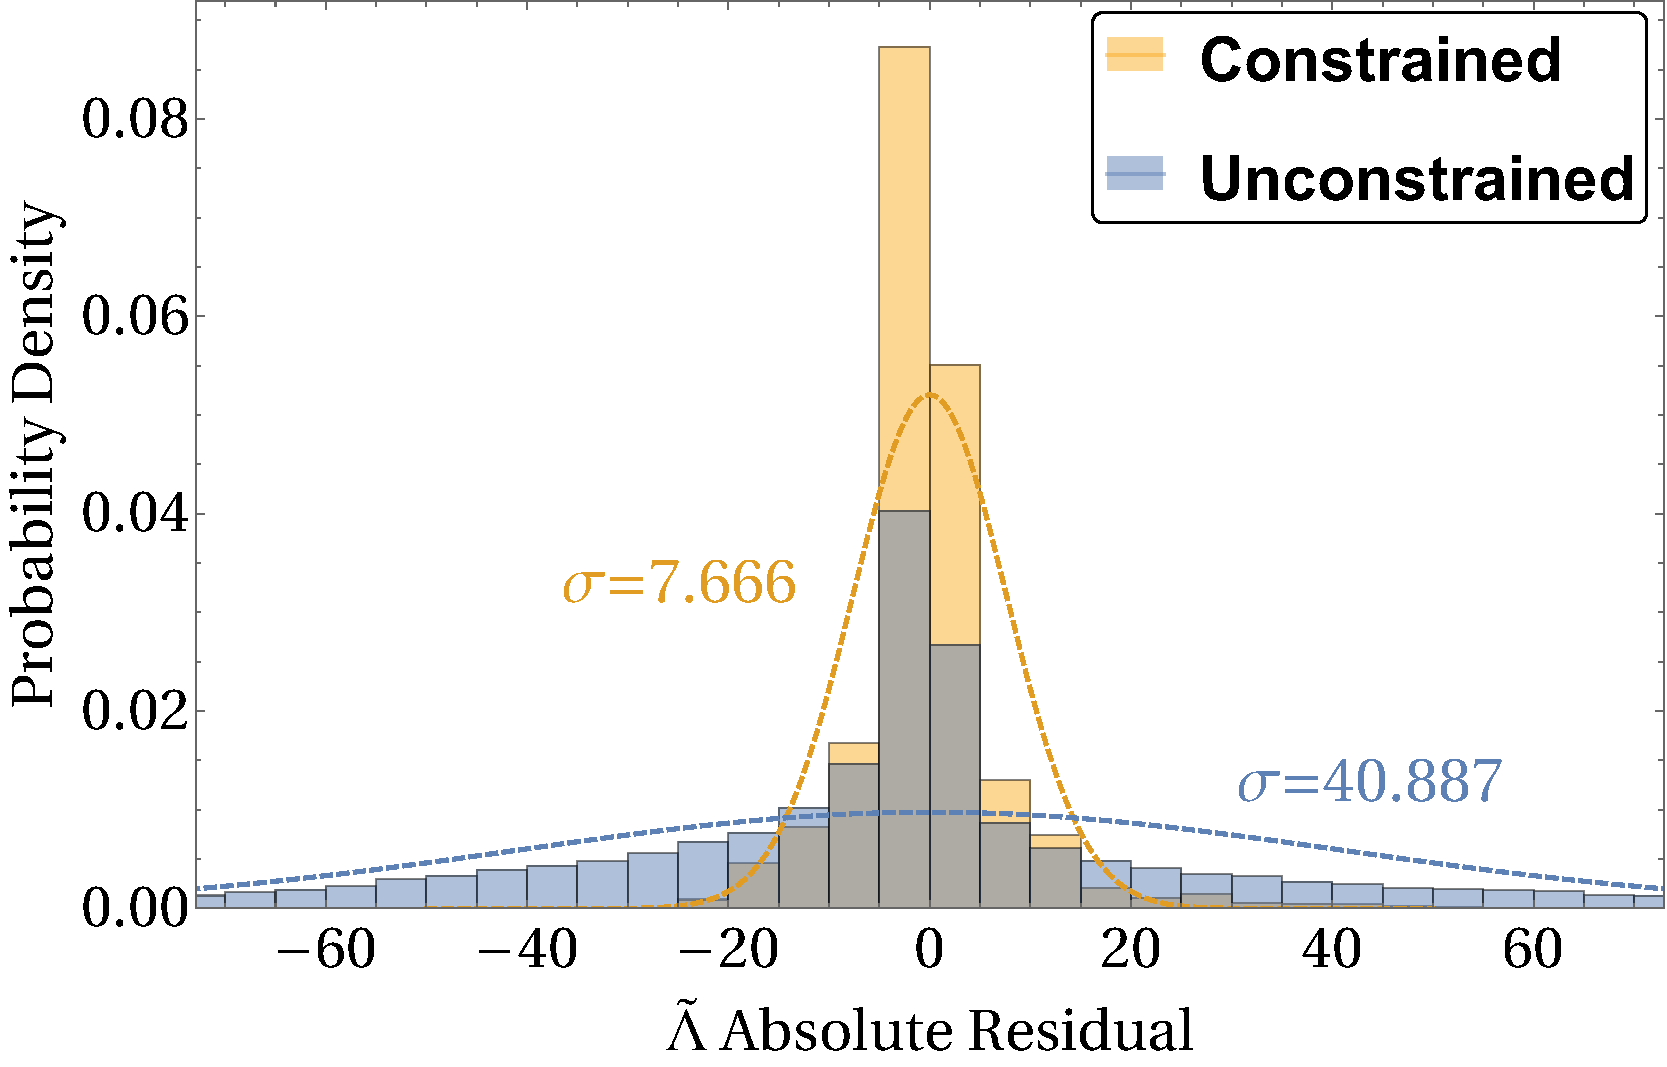
\includegraphics[width=\columnwidth]{residuals.pdf}
\end{center}
\caption{
Residuals on $\lambda_0$ computed as $\lambda_0^{\text{fit}}-\lambda_0^{\text{true}}$ for the binary Love relations modeled in Sec.~\ref{sec:binLove-nuclear} for both constrained and unconstrained sets of EoSs.
These residuals obey Gaussian distributions centered at $\mu=-2.39 \times 10^{-27} \text{ s}^5$ and $\mu=4.22 \times 10^{-27} \text{ s}^5$ with standard deviations of $\sigma=1.52\times10^{-25} \text{ s}^5$ and $\sigma=12.21\times10^{-25} \text{ s}^5$ for the constrained and unconstrained sets of EoSs, respectively.
These uncertainties correspond roughly to the systematic errors introduced on the parameter extraction of $\lambda_0$ upon the use of binary Love relations.
However, to take into account the systematic errors found in high-error regions of the parameter space, we instead set the systematic error to be the 90th percentile, $P_{90}=2.06\times10^{-25} \text{ s}^5$.
Observe that the systematic errors from using the improved (constrained) binary Love relations are negligible compared to the statistical errors accrued on parameter extraction from GW170817, found to be $\sigma_{\lambda_0}=26.53 \times 10^{-25} \text{ s}^5$.
}
\label{fig:residuals}
\end{figure}

%%%%%%%%%%%%%%%%%%%%%%%%% Begin Future Observations %%%%%%%%%%%%%%%%%%%%%%%%%%%%%%%%%%%%%%%%%%%%%%%%%%%%%%%%%%%%%%%%%%%%%%%%%%%%%%%%%%%%%%%%%%%%%%%%%%%%%%%%%%%%%%%%%%%%%%%%%%%%%%%%%%%%%%%%%%%%%%%%%%%%%
\section{Impact on future observations}\label{sec:observations}
In this section, we estimate the feasibility of utilizing improved EoS-insensitive relations in future binary NS merger events.
This estimate is acquired through a simple Fisher analysis~\cite{Finn:Fisher,Cutler:Fisher} which approximates the accuracy with which one can extract best-fit parameters $\theta^a$, given a prior template waveform.
For the remainder of the paper, we consider a template parameter vector consisting of:
\begin{equation}\label{eq:template}
\theta^a=(\ln{A},\phi_c,t_c,\ln{\mathcal{M}},\ln{\mathcal{\eta}},\chi_s,\chi_a,\lambda_0, \lambda_1),
\end{equation}
where $A \equiv \sqrt{\frac{2 \eta}{3 \pi^{1/3}}}$ is a normalized amplitude factor, $\eta \equiv m_1 m_2/M^2$ is the symmetric mass ratio with $m_{1,2}$ and $M$ being the individual and total masses, $\mathcal{M}=M \eta^{3/5}$ is the chirp mass, and $\chi_{s,a}=\frac{1}{2}(\chi_1\pm\chi_2)$ are the symmetric and antisymmetric total spins, where $\chi_{1,2}$ are the NSs individual spins. 
Following Refs.~\cite{Cutler:Fisher,Berti:Fisher,Poisson:Fisher}, this method relies on the crude assumption of Gaussian prior distributions\footnote{Typically, the more valid assumption is a uniform prior distribution; an improvement made in a more detailed Bayesian analysis.}.
The resulting posterior distribution is Gaussian with root-mean-square given by:
\begin{equation}
\Delta \theta^a=\sqrt{\Big( \tilde{\Gamma}^{-1}\Big)^{aa}}.
\end{equation}
Here, the Fisher matrix $\tilde{\Gamma}$ is defined by:
\begin{equation}
\tilde{\Gamma}_{ab} \equiv \Big( \frac{\partial h}{\partial \theta^a} \Big| \frac{\partial h}{\partial \theta^a}\Big) + \frac{1}{\sigma_{\theta^a}^2} \delta_{ab}
\end{equation}
where $h$ is the waveform template, $\sigma_{\theta^a}$ is the parameters' prior root-mean-square estimate, and the inner product is defined by:
\begin{equation}
(a|b) \equiv 2 \int^{\infty}_0\frac{\tilde{a}^*\tilde{b}+\tilde{b}^*\tilde{a}}{S_n(f)}df.
\end{equation}

In this analysis, we consider the ``PhenomD" (IMRD) waveform template~\cite{PhenomDI,PhenomDII} modified by two different tidal corrections: the 6PN tidal correction shown in Ref.~\cite{Wade:tidalCorrections} (IMRD + 6PN), and the NRTidal correction shown in Ref.~\cite{Samajdar:NRTidal} (IMRD + NRTidal).
Comparing the two tidal corrections to the IMRD waveform returns an estimate on the magnitude of waveform mismodeling systematics.
Lastly, we consider the spectral noise density $S_n^A(f)$ for 6 different interferometer designs: $A \equiv ($O2~\cite{aLIGO}, aLIGO~\cite{aLIGO}, A\texttt{+}~\cite{Ap_Voyager_CE}, Voyager~\cite{Ap_Voyager_CE}, CE~\cite{ET}, ET-D~\cite{Ap_Voyager_CE}$)$ in order to compare the statistical errors accrued on parameter extraction using future upgraded detectors.

We begin by authenticating this approach by applying a Fisher analysis (IMRD + 6PN waveform injection) to GW170817, as observed by LIGO with O2 detector sensitivity~\cite{aLIGO}.
Because only 1 event was detected, we utilize $\tilde\Lambda$ and $\delta\tilde\Lambda$ as the tidal parameters for comparison purposes.
Further, we scale the luminosity distance such that the signal-to-noise-ratio ($SNR \equiv \rho$) is fixed to be $\rho=32.4$, as was found in GW170817.
We also assume low spin priors $|\chi| \leq 0.05$, as well as $\tilde{\Lambda} \leq 3000$ and $|\delta \tilde{\Lambda}| \leq 500$~\cite{Wade:LambdaPriors}.
The resulting posterior distribution on $\tilde{\Lambda}$ has a range of $\pm 276.99$ encompassing the $90\%$ credible levels.
We compare these results with the Bayesian analysis performed in Ref.~\cite{TheLIGOScientific:2017qsa,Abbott2018}, finding close agreement with the resulting $90\%$ credible region of $70 \leq \tilde{\Lambda} \leq 720$.
This confirms the approximate validity of this method, allowing a continuation of this analysis for future detectors.
\begin{figure}
\begin{center} 
\includegraphics[width=\columnwidth]{sensitivities.eps}
\end{center}
\caption{
Square root of of the spectral noise densities $\sqrt{S_n^A(f)}$ plotted for detectors ($A$): LIGO O2 (orange), aLIGO (green), A\texttt{+} (purple), Voyager (magenta), CE (red), and ET-D (blue) as interpolated from publicly available data.
Spectral noise densities are plotted from $f_{\text{min}}=(23,10,10,7,1,1) \text{ Hz}$, respectively, to $f_{\text{max}}=1649 \text{ Hz}$.
Also shown is $2 \sqrt{f}$ multiplied by the amplitude of the PhenomD~\cite{PhenomDI,PhenomDII} waveform template.
}
\label{fig:sensitivities}
\end{figure}

Next, we consider events identical to GW170817 detected on future design sensitivity upgrades and detectors $A \equiv ($O2, aLIGO, A\texttt{+}, Voyager, CE, ET-D$)$, shown in Fig.~\ref{fig:sensitivities}, to determine if and when the statistical errors associated with parameter extraction of $\lambda_0$ drop below the systematic EoS variation errors from using binary Love relations.
The process we use for each detector sensitivity $S_n^A(f)$ is as follows:
\begin{itemize}
\item Perform a Fisher analysis as outlined above using $S_n^A(f)$, while restricting the luminosity distance $D_L$ such that $\rho^{\text{O2}}_{\text{GW170817}}=32.4$ would be achieved on O2 sensitivity $S_n^{\text{O2}}(f)$.
Here we assume low spin priors $|\chi| \leq 0.05$, as well as $0 \text{ s}^5 \leq \lambda_0 \leq 5 \times 10^{-23} \text{ s}^5$ and $-5 \times 10^{-18} \text{ s}^4\text{ M}_{\odot} \leq \lambda_1 \leq 0 \text{ s}^4\text{ M}_{\odot}$~\cite{delPozzo:TaylorTidal}.
This results in SNR $\rho^A_{\text{GW170817}}$ and statistical error $\sigma_\text{GW170817}^A$ accrued in the extraction of $\lambda_0$ on detector $A$.
\item Generate a population of $N_A$ events corresponding to the expected binary NS merger detection rate for detector $A$, following the distribution $f=3 \rho_{\text{th}}^3/\rho^4$~\cite{Shutz:SNR,Chen:SNR} with a network SNR threshold of $\rho_{\text{th}}=8$.
The number of events $N_A$ is calculated by taking into account the BNS merger rate history throughout all redshift values within detector As' horizon distance $z_h$, as shown by Eq. (10) of Ref.~\cite{Cutler:BNSmerger}:
\begin{equation}
N_A=\Delta \tau_0 \int\limits^{z_{h}}_0 4 \pi \lbrack  a_0r_1(z)\rbrack^2 \mathcal{R} r(z) \frac{d \tau}{dz} dz.
\end{equation}
Here, $a_0r_1(z)$, $\frac{d\tau}{dz}$, and $r(z)$ for our chosen cosmology are given by:
\begin{equation}
a_0r_1(z) = \frac{1}{H_0}\int\limits^z_0 \frac{dz'}{\sqrt{(1-\Omega_{\Lambda})(1+z')^3+\Omega_{\Lambda}}},
\end{equation}
\begin{equation}
\frac{d\tau}{dz} = \frac{1}{H_0} \frac{1}{1+z}\frac{1}{\sqrt{(1-\Omega_{\Lambda})(1+z')^3+\Omega_{\Lambda}}},
\end{equation}
\begin{equation}
r(z) = \left\{
\begin{array}{ll}
      1+2z & z \leq 1 \\
      \frac{3}{4}(5-z) & 1\leq z\leq 5 \\
      0 & z\geq 5\\ 
\end{array} 
\right.
\end{equation}

where $H_0 = 70 \text{km s}^{-1}\text{Mpc}^{-1}$ is the local Hubble constant, and $\Omega_{\Lambda}=0.67$ is the universe's vacuum energy density.
Here we choose an observing period $\Delta \tau = 1$ year {\ny{Should this be tau 0?}}, and calculate the detection rate for the upper, central, and lower limits of the local binary NS coalescence rate density $\mathcal{R}=1540^{+3200}_{-1220} \text{ Gpc}^{-3}\text{yr}^{-1}$~\cite{Abbott2017}, giving the rates shown in the second column of Table~\ref{tab:variances}.
\item Compute the overall population standard deviation, taking into account sources at varying redshifts as done in Eq. (3) of Ref.~\cite{Takahiro}:
\begin{equation}
\sigma_{N_A}^{-2}=\Delta \tau \int\limits^{z_h}_04 \pi \lbrack a_0 r_1(z)\rbrack^2 \mathcal{R}r(z)\frac{d\tau}{dz}\sigma^A_i(z)^{-2}dz
\end{equation}
where $\sigma_i^A(z)$ is computed by the relations $\sigma_i^A \times \rho_i^A = \sigma_{\text{GW170817}}^A \times \rho_{\text{GW170817}}^A$.
\item \zc{These bullet points are getting kind of long and detailed. They (at least the low-level version of them) could go in a new appendix section - let me know what everyone thinks :)}
\end{itemize}

{\ny{I think you need more detail because I didn't understand how you computed the combined statistical error. Perhaps you could give a concrete example of 1 iteration of the method, say if N = 2. This could make it much clearer and yes, you could move all of this to an appendix. }}

The results for this process upon the injection of the IMRD + 6PN waveform are compiled in Table~\ref{tab:variances}, and shown graphically in Fig.~\ref{fig:stackedFisher} where $\sigma^A_{\text{GW170817}}$ and $\sigma^A_N$ are plotted as a function of $\rho^A_{\text{GW170817}}$ (the SNR as if GW170817 were detected on future detector $A$) for 5 future detector sensitivities.
For reference, Fig.~\ref{fig:singleFisherLt} also displays the estimated $\tilde\Lambda$ extraction efficiency for \emph{one} event on each detector; as these events can not be combined like was done in the case of $\lambda_0$.
Observe how this figure shows similar results on $\tilde\Lambda$ to that found on $\lambda_0$ for the case of one event - that is, future detectors ET and CE both observe statistical errors on $\tilde\Lambda$ dropping below the systematic binary Love errors for a single event.
\begin{figure}
\begin{center} 
\includegraphics[width=\columnwidth]{singleFisherLt.eps}
\end{center}
\caption{
Estimated statistical uncertainties $\sigma^A_{\text{GW170817}}$ (blue) in the extraction of $\tilde\Lambda$ from GW170817 (O2) as if observed with future interferometers aLIGO, A\texttt{+}, Voyager, CE, and ET-D as a function of the signal-to-noise-ratio $\rho^A_{\text{GW170817}}$.
Also shown is the systematic error on $\tilde\Lambda$ (indigo) derived using the same method used to compute the systematic error on $\lambda_0$.
This is similar to Fig.~\ref{fig:stackedFisher} where the extraction efficiency of $\lambda_0$ was plotted.
However, in this case multiple events can \emph{not} be combined due to the variation in mass and therefore $\tilde\Lambda$ among events.
}
\label{fig:singleFisherLt}
\end{figure} 

\begin{table*}
\centering
\caption{
Tabulated results for the estimated statistical errors on $\lambda_0$ for the combined results of $N_A$ detections corresponding to the estimated upper, central, and lower limits of the binary NS merger detection rate $R$.
This is repeated for 5 future detector sensitivities: aLIGO, A\texttt{+}, Voyager, CE, and ET.
Below, $\rho^A_{\text{GW170817}}$ and $\sigma^A_{\text{GW170817}}$ correspond to the approximate SNR and $\sigma_{\lambda_0}$ of GW170817 had it been observed by the future interferometer, and $\sigma^A_N$ corresponds to the final uncertainty on $\lambda_0$ after $N_A$ detections on interferometer $A$.
It can be seen here that the statistical errors on $\lambda_0$ become comparable with the systematics (set to be $P_{90}=12.014$) from using improved binary Love relations from Voyager and on, indicating when it may be safe to utilize new EoS-insensitive relations.
Note the approximation for $\sigma^A_N$ under the O2 detector sensitivity is left blank due to the singularity of the detected event.
These results are shown graphically in Fig.~\ref{fig:stackedFisher}.
}\label{tab:variances}
\begin{tabular}{|c|@{\extracolsep{4pt}}c@{\extracolsep{0pt}}|c|@{\extracolsep{4pt}}C{1.7cm}@{\extracolsep{-2pt}}|C{1.7cm}|@{\extracolsep{-2pt}}C{1.7cm}@{\extracolsep{2pt}}|c|@{\extracolsep{0pt}}c@{\extracolsep{0pt}}|c|}
\cline{1-1}\cline{2-3}\cline{4-9}
    \multicolumn{1}{|c|}{\bfseries Detectors (A)} & \multicolumn{2}{|c|}{\bfseries GW170817} & \multicolumn{6}{|c|}{\bfseries Multiple events} \\
\cline{1-1}\cline{2-3}\cline{4-9}
\noalign{\smallskip}
\cline{2-3}\cline{4-6}\cline{7-9}
\multicolumn{1}{c}{} & \multicolumn{1}{|c|}{} & \multicolumn{1}{c|}{} & \multicolumn{3}{|c|}{} & \multicolumn{3}{|c|}{}
\\[-1em]
\multicolumn{1}{c}{}  &  \multicolumn{1}{|c|}{\multirow{2}{*}{$\rho^A_{\text{GW170817}}$}}  &  \multirow{ 2}{*}{\large $\frac{\sigma^A_{\text{GW170817}}}{10^{-25}}$}  &  \multicolumn{3}{|c|}{$N_A$}  &  \multicolumn{3}{|c|}{$\sigma^A_N / 10^{-25}$}  \\
\cline{4-6}\cline{7-9}
\multicolumn{1}{c}{}  &  \multicolumn{1}{|c|}{}  &  \multicolumn{1}{c|}{}  &  \multicolumn{1}{|c|}{Low}  &  \multicolumn{1}{c|}{Central} &  \multicolumn{1}{c|}{High}  & \multicolumn{1}{|c|}{Low}  &  \multicolumn{1}{c|}{Central} &  \multicolumn{1}{c|}{High}\\
\cline{2-3}\cline{4-6}\cline{7-9}
\noalign{\smallskip}
\noalign{\smallskip}
\cline{1-1}\cline{2-3}\cline{4-6}\cline{7-9}
 O2  & \multicolumn{1}{|c|}{$32.40$}  & $26.53$ &  \multicolumn{1}{|c|}{--} & -- & -- & \multicolumn{1}{|c|}{--} & -- & --\\
\cline{1-1}\cline{2-3}\cline{4-6}\cline{7-9}
 aLIGO  & \multicolumn{1}{|c|}{$90.74$}  & $17.10$ &  \multicolumn{1}{|c|}{$20$} & $98$ & $304$ & \multicolumn{1}{|c|}{$28.51$} & $12.99$ & $7.32$\\
\cline{1-1}\cline{2-3}\cline{4-6}\cline{7-9}
 A\texttt{+}  & \multicolumn{1}{|c|}{$180.95$}  & $7.12$ &  \multicolumn{1}{|c|}{163} & 786 & 2,419 & \multicolumn{1}{|c|}{$9.19$} & $3.85$ & $2.13$\\
\cline{1-1}\cline{2-3}\cline{4-6}\cline{7-9}

\multicolumn{1}{|c|}{} & \multicolumn{1}{|c|}{} & \multicolumn{1}{c|}{} & \multicolumn{1}{|c|}{} & \multicolumn{1}{c|}{} & \multicolumn{1}{c|}{} & \multicolumn{1}{|c|}{} & \multicolumn{1}{c|}{} & \multicolumn{1}{c|}{}
\\[-1em]

 Voyager  & \multicolumn{1}{|c|}{$428.89$}  & $3.94$ &  \multicolumn{1}{|c|}{2,191} & 10,544 & 32,454 & \multicolumn{1}{|c|}{$3.27$} & $1.49$ & $0.83$\\
\cline{1-1}\cline{2-3}\cline{4-6}\cline{7-9}

\multicolumn{1}{|c|}{} & \multicolumn{1}{|c|}{} & \multicolumn{1}{c|}{} & \multicolumn{1}{|c|}{} & \multicolumn{1}{c|}{} & \multicolumn{1}{c|}{} & \multicolumn{1}{|c|}{} & \multicolumn{1}{c|}{} & \multicolumn{1}{c|}{}
\\[-1em]

 ET-D  & \multicolumn{1}{|c|}{$1398.03$}  & $1.07$ &  \multicolumn{1}{|c|}{71,536} & 344,270 & 1,059,638 & \multicolumn{1}{|c|}{$0.60$} & $0.27$ & $0.15$\\
\cline{1-1}\cline{2-3}\cline{4-6}\cline{7-9}

\multicolumn{1}{|c|}{} & \multicolumn{1}{|c|}{} & \multicolumn{1}{c|}{} & \multicolumn{1}{|c|}{} & \multicolumn{1}{c|}{} & \multicolumn{1}{c|}{} & \multicolumn{1}{|c|}{} & \multicolumn{1}{c|}{} & \multicolumn{1}{c|}{}
\\[-1em]

 CE  & \multicolumn{1}{|c|}{$2807.45$}  & $1.20$ &  \multicolumn{1}{|c|}{295,200} & 1,420,650 & 4,372,653 & \multicolumn{1}{|c|}{$0.58$} & $0.26$ & $0.14$\\
\cline{1-1}\cline{2-3}\cline{4-6}\cline{7-9}
\end{tabular}
\end{table*}

Next, we repeat the process upon the injection of the IMRD + NRTidal waveform in order to demonstrate the effect of waveform mismodeling.
The results are shown in Fig.~\ref{fig:stackedFisher} by blue outlined circles (single detection uncertainties) and the outlined dashed maroon region (combined uncertainties from multiple detections).
Observe the noticeable difference between the extraction efficiencies for the two different tidal corrections - highlighting the need for further waveform modeling for future interferometers.

{\ny{Super confused about Fig. 1...}}

Concluding, we find that the Voyager, ET, and CE detectors all exhibit enough uncertainty reduction that the systematics on $\lambda_0$ introduced from using improved EoS-insensitive relations (found to be $2.06 \times 10^{-25}\text{ s}^5$) no longer become negligible in the error budget.
This was also shown for the case of $\tilde\Lambda$, only taking into account single observed events, where ET and CE detectors both observe comparable statistical and systematic errors on $\tilde\Lambda$.
This implies that the use and further improvement of EoS-insensitive relations is not only justified, but necessary, for future binary NS merger detections.
Further, we investigate the dependence of the measurement accuracy of $\tilde\Lambda$ on the binary NS mass ratio $q$ for fixed chirp mass $\mathcal{M}=1.88\text{ M}_{\odot}$ in Appendix~\ref{app:measurement}.

%%%%%%%%%%%%%%%%%%%%%%%%% Begin Discussion %%%%%%%%%%%%%%%%%%%%%%%%%%%%%%%%%%%%%%%%%%%%%%%%%%%%%%%%%%%%%%%%%%%%%%%%%%%%%%%%%%%%%%%%%%%%%%%%%%%%%%%%%%%%%%%%%%%%%%%%%%%%%%%%%%%%%%%%%%%%%%%%%%%%%
\section{Conclusion and Discussion}\label{sec:conclusion}
The recent GW observation of binary NS merger GW170817 placed constraints on the supranuclear matter EoS for NSs.
We take advantage of this by generating a restricted set of spectral EoSs which agree with this observation to reduce uncertainties upon the extraction of tidal parameters from future GW events.
Important previous work by Yagi and Yunes~\cite{Yagi:ILQ,Yagi:binLove} found EoS-insensitive relations between symmetric and antisymmetric combinations of NS tidal deformabilities, which aid in the extraction of said tidal parameters.
We find an improvement upon these EoS-insensitive relations by a factor of $\sim 59$\% for stars with mass ratios of $0.75$ by restricting to the EoS posterior samples from GW170817s 90\% credible region on pressure as a function of density.
Similarly, we find an increase in C-Love and I-Love-Q universality by a factors of $\sim 76$\% and $\sim 50$\%, respectively.
We also show new R-Love relations relating the NS radius to its tidal deformability, displaying a maximum of $18.88\%$ EoS variability from the fit discussed in Sec.~\ref{sec:clove}.
Additionally, we find that hybrid quark-hadron star EoSs \emph{do} obey the I-Love-Q and C-Love universality, albeit with a slightly higher maximum EoS variability as displayed in Tabs.~\ref{tab:hybridCompare} and ~\ref{tab:hybridCompareClove}.
In addition, we find that binaries consisting of one massive hybrid quark-hadron star, and one small-mass hadron star do not obey the binary Love relations -- explained by the large difference in $\tilde{\Lambda}$ displayed between the constituent stars.
To improve on this, we construct new ``hybrid matter binary Love relations", applied to only the hybrid branches of the transitional EoSs.
This results in EoS variability similar to that found for the nuclear matter fits.
Further, we analyze the impact of this improvement for future binary NS merger detections, as the current detector sensitivity is not yet small enough to accurately constrain $\tilde{\Lambda}$ enough for EoS-insensitive relations to make a difference.
We find that future interferometers Voyager, CE, and ET-D all experience statistical uncertainties upon the extraction of $\tilde{\Lambda}$ small enough to become comparable to the systematic errors injected through the use of improved EoS-insensitive relations (found to be $12.014$), as depicted in Fig.~\ref{fig:stackedFisher} and Table~\ref{tab:variances}.
Additionally, we considered the effect of waveform mismodeling by comparing Fisher analyses using two different tidal corrections to the PhenomD waveform: 6PN and NRTidal.
Doing so revealed a noticeable difference between the extraction uncertainties derived under injection of each waveform - indicating the need for further waveform modeling.
Finally, in Appendix~\ref{app:measurement} we investigate the effect of NS binary mass ratio q on the measurement accuracy of $\tilde\Lambda$.
We find that second generation interferometers lose accuracy as one increases the mass ratio, while third generation detectors observe a large increase of accuracy due to the correlations between $\tilde\Lambda$ and $\delta\tilde\Lambda$.
This indicates that the use and further improvement of EoS-insensitive relations is justified for future GW observations of binary NS merger events.

Future work on this subject entails an investigation into the improvement of alternative EoS insensitive relations, such as the multipole Love relations between various $l$-th order electric, magnetic, and shape tidal deformabilities as discussed in Ref.~\cite{Yagi:Multipole}.
Additionally, Lackey \emph{et al}. presented surrogate models of non-spinning effective-one-body waveform models with the the use of universal relations in Refs.~\cite{Lackey:Surrogate, Lackey:EOB}.
By reducing the number of required waveform model parameters, surrogate models aid in the extraction of NS observables from GW detections.
The improvement of multipole love relations can then be used to increase the accuracy of surrogate models.

%%%%%%%%%%%%%%%%%%%%%%%%% Begin Acknowledgements %%%%%%%%%%%%%%%%%%%%%%%%%%%%%%%%%%%%%%%%%%%%%%%%%%%%%%%%%%%%%%%%%%%%%%%%%%%%%%%%%%%%%%%%%%%%%%%%%%%%%%%%%%%%%%%%%%%%%%%%%%%%%%%%%%%%%%%%%%%%%%%%%%%%%
\section*{Acknowledgments}\label{acknowledgments}
K.Y. would like to acknowledge networking support by the COST Action GWverse CA16104.

%%%%%%%%%%%%%%%%%%%%%%%%% Begin Appendix A: measurement accuracy as a functino of q %%%%%%%%%%%%%%%%%%%%%%%%%%%%%%%%%%%%%%%%%%%%%%%%%%%%%%%%%%%%%%%%%%%%%%%%%%%%%%%%%%%%%%%%%%%%%%%%%%%%%%%%%%%%%%%%%%%%%%%%%%%%%%%%%%%%%%%%%%%%%%%%%%%%%
\appendix
\section{Measurement accuracy as a function of binary mass ratio}\label{app:measurement}
In this appendix, we discuss the effects of the binary NS mass ratio on the measurement accuracy of $\tilde\Lambda$ for various interferometers. 
The left panel of Fig.~\ref{fig:massVariation} displays an approximation of the $\tilde\Lambda$ measurement accuracy as a function of increasing mass ratio $q$ (for a fixed chirp mass of $\mathcal{M}=1.188 \text{ M}_{\odot}$ corresponding to GW170817), using the Fisher analysis techniques described in Sec.~\ref{sec:observations}.
We observe two points of interest about these trends: (i) the second generation detectors (O2, aLIGO, A\texttt{+}, and Voyager) typically become less accurate as the mass ratio approaches unity, (ii) the third generation detectors (CE and ET) observe the opposite behavior-- a fast growth in accuracy as the mass ratio increases.
For the remainder of this appendix, we attempt to explain the opposing behaviors of the second and third generation interferometers on the extraction of $\tilde\Lambda$.

\begin{figure}
\begin{center} 
\includegraphics[width=.3\textwidth]{massVariation1.eps}
\includegraphics[width=.3\textwidth]{massVariation2.eps}
\includegraphics[width=.3\textwidth]{massVariation3.eps}
\end{center}
\caption{
Measurement accuracy of $\tilde\Lambda$ as a function of increasing mass ratio $q$ for interferometer sensitivities O2, aLIGO, A\texttt{+}, Voyager, CE, and ET.
Evaluated at a fixed chirp mass of $\mathcal{M}=1.188\text{ M}_{\odot}$ corresponding to GW170817, this is repeated for three cases: (i) (top) with correlations between all template waveform parameters $\theta^a$ intact; (ii) (center) with the correlations between $\tilde\Lambda$ and $\delta\tilde\Lambda$ removed; and (iii) (bottom) with correlations between all parameters removed.
The removal of parameter correlations is approximated by setting certain Fisher matrix elements to 0, as described in Appendix.~\ref{app:measurement}.
Observe how the left panel shows strong disagreement between second and third generation detectors, while the right panel shows identical behavior.
This indicates that parameter correlations between $\tilde\Lambda$ and higher PN order parameter $\delta\tilde\Lambda$ to be the culprit in such a disagreement.
}
\label{fig:massVariation}
\end{figure} 

We begin by considering the correlations between individual template parameters and $\tilde\Lambda$, given in Eq.~\ref{eq:template}.
A simple approximation on the amplitude of these correlations can be performed by assuming all other correlations are non-existing.
Correlations between parameters $\tilde\Lambda$ and $\theta^a$ alone is achieved by setting all off-diagonal Fisher matrix elements to $0$, except for the $(i,j)$ components such that both $i$ and $j$ correspond to the $\tilde\Lambda$ and $\theta^a$ parameters.
We follow this process for each parameter in turn, and display the results in Fig.~\ref{fig:correlations} for each interferometer.
This figure, showing only the relative differences between correlations of different parameters $\theta^a$ and $\tilde\Lambda$, reveals a few things.
First, the coalescence time $t_c$ is highly correlated with $\tilde\Lambda$ equally for each interferometer, an unsurprising fact due to the high 4PN order at which the parameter enters the waveform.
Secondly, correlations with 6PN tidal parameter $\delta\tilde\Lambda$ shows high correlations with $\tilde\Lambda$ for only the third generation detectors.
This can be explained by the high PN order at which $\delta\tilde\Lambda$ enters the waveform, an effect that only the most sensitive of detectors can probe. 

\begin{figure}
\begin{center} 
\begin{overpic}[width=\columnwidth]{correlations.eps}
\put(121,13){\fontsize{7pt}{7pt}\selectfont $\mathcal{M}$}
\end{overpic}
\end{center}
\caption{
Measurement accuracy of $\tilde\Lambda$ upon the consideration of correlations between \emph{only} $\tilde\Lambda$ and other individual template parameters $\theta^a$ shown in Eq.~\ref{eq:template}.
This process, repeated for 6 interferometer design sensitivities O2, aLIGO, A\texttt{+}, Voyager, CE, and ET, is approximated by setting all off-diagonal Fisher matrix elements to 0 except for the $(i,j)$ components such that both $i$ and $j$ correspond to the $\tilde\Lambda$ and $\theta^a$ parameters.
Observe how correlations with 4PN parameter $t_c$ (coalescence time) remain to be highly correlated with $\tilde\Lambda$ among all 6 interferometers.
However, correlations between 6PN tidal parameter $\delta\tilde\Lambda$ and $\tilde\Lambda$ only begin to make a strong impact for third generation detectors.
This is due to the small effect that $\delta\tilde\Lambda$ has on the waveform, only to be distinguished by the most sensitive detectors.
}
\label{fig:correlations}
\end{figure} 

Following this conclusion on the difference of correlations between tidal parameters $\tilde\Lambda$ and $\delta\tilde\Lambda$ for second and third generation detectors, we attempt to describe the opposing behaviors of measurement accuracy between the two.
Shown in the center panel of Fig.~\ref{fig:massVariation}, we approximate the measurement accuracy of $\tilde\Lambda$ with the correlations between $\delta\tilde\Lambda$ and $\tilde\Lambda$ removed, through a process similar to that described above. 
Notice how the trends between detector generations become more similar -- implying that the correlations between tidal parameters may be the cause.
This is confirmed by the right panel of Fig.~\ref{fig:massVariation} where all parameter correlations have been removed from the Fisher matrix.
We see that this results in identical behaviors between all 6 representative interferometers, leading us to conclude that the discrepancy between interferometers comes from the degeneracies between different parameters in the gravitational waveform, namely the 6PN tidal parameter $\delta\tilde\Lambda$ which is only detectable by the highly sensitive third generation detectors CE and ET.

%%%%%%%%%%%%%%%%%%%%%%%%% Begin Bibliography  %%%%%%%%%%%%%%%%%%%%%%%%%%%%%%%%%%%%%%%%%%%%%%%%%%%%%%%%%%%%%%%%%%%%%%%%%%%%%%%%%%%%%%%%%%%%%%%%%%%%%%%%%%%%%%%%%%%%%%%%%%%%%%%%%%%%%%%%%%%%%%%%%%%%%
\clearpage
\bibliography{Zack}
\end{document}

